\documentclass[11pt]{article}
\usepackage[margin=1in]{geometry}
\usepackage{amsmath,amssymb}
\usepackage{graphicx}
\usepackage{booktabs}
\usepackage{float}
\usepackage{array}
\usepackage[hidelinks]{hyperref}
\usepackage{enumitem}
\setlist{nosep,leftmargin=1.6em}
\newcommand{\degrees}{\ensuremath{^\circ}}
\newcommand{\DHR}{\text{DHR}}
\graphicspath{{../figures/}}
\setlength{\parskip}{2pt}
\setlength{\emergencystretch}{1.5em}
\title{\textbf{Air Conditioning the Environment:\\ Delivering Cooling Where It Counts}}
\author{HiMCM 2026 -- Problem B \quad$\cdot$\quad Team \#TBD \quad$\cdot$\quad November 2026}
\date{}

\begin{document}
\maketitle
\vspace{-4em}

%=====================================================================
\section*{Summary Sheet}
\addcontentsline{toc}{section}{Summary Sheet}
%=====================================================================
\textbf{Problem.} Open-air venues and semi-open public spaces spend electricity cooling air that partly escapes to the atmosphere. We build a general framework to measure how much \emph{useful} cooling systems deliver and to balance comfort, safety, energy, and cost across venues and climates.

\noindent\textbf{Approach.} The open freezer case teaches the central lesson: efficiency is \emph{useful cooling delivered at the person} divided by \emph{energy consumed} --- not energy use alone. We construct a four-layer framework:
\begin{enumerate}
\item \textbf{Physics:} psychrometric wet-bulb temperature; evaporative drop $\Delta T=\min(\Delta T_{\mathrm{rated}},\,0.85\,(T_{db}-T_{wb}))$; humidity-corrected perceived fan cooling; a transient heat-balance ODE for semi-open halls.
\item \textbf{People:} perceived temperature, comfort caps (relief only counts above $27\degrees$C), and a WBGT-based heat-strain safety model.
\item \textbf{Efficiency:} the \textbf{Degree-Hours of Relief per kWh} metric, $\DHR = \sum N_{\text{served}}\cdot r\,/\,\mathrm{kWh}$ (person-$\degrees$C$\cdot$h per kWh), plus thermodynamic and cost cross-checks.
\item \textbf{Effectiveness:} a hard service floor ($\geq$80\% of person-time acceptable) combined with a weighted four-objective score and Pareto analysis.
\end{enumerate}

\noindent\textbf{Key results.}
\begin{itemize}
\item \textit{Bus stop (Req.~2a):} the fan is the efficiency champion (96 vs.\ 50 and 38.4 person-$\degrees$C$\cdot$h/kWh for fan, evaporative, and large evaporative in dry heat), \emph{but} at $41\degrees$C only the large evaporative cooler keeps a served person below heat-strain levels. The most efficient choice is not the safest.
\item \textit{Rail station (Req.~2b):} the transient zonal model (thermal mass, surges, safety, economics) shows that a grid-optimised hybrid policy --- fans always on; the evaporative fleet behind a robust $27.5$--$30\degrees$C thermostat with pre-cooling --- delivers $\approx$100\% acceptable person-time at 43--50\% less energy than always-on operation (95.8 vs.\ 169.5 kWh/day in dry heat), and stays feasible in $\geq$98.8\% of 400 Monte-Carlo plant-uncertainty draws.
\item \textit{Effectiveness (Req.~4):} under the hard service floor, no-cooling and fans-only options are infeasible in both climates; the hybrid wins in hot-arid (0.729) and hot-humid (0.613) climates, ranking first under 400/400 and 358/400 random weight draws. In humid heat, refrigerative cooling becomes a robust competitor (feasible in every humid draw); in dry heat it fails in every draw.
\item \textit{Scaling (Req.~3):} the same equations transfer unchanged across four venues in four climates; occupancy density, rated drop and power dominate dry-heat sensitivity, while humidity and the comfort cap govern humid heat (large-cooler $\DHR$ collapses from 213 in Phoenix to 10 in Singapore).
\end{itemize}

\noindent\textbf{Recommendations.} Cool the person, not the space: shade and fans first; evaporative cooling in dry climates; refrigeration where recirculation is possible in humid ones; the Monte-Carlo-robust thermostat policy (43--50\% energy saving). In extreme heat, switch to always-on: efficiency yields to safety.

\newpage
%=====================================================================
\tableofcontents
\newpage
%=====================================================================
\section{Introduction and Restatement}
%=====================================================================
Public cooling in spaces that are not fully enclosed --- stadium concourses, amphitheaters, transit stations, airport terminals, waiting areas --- resembles an open freezer case: cold air escapes, warm air enters, and the plant works against the whole atmosphere \cite{comap}. As heat waves intensify, operators must decide \emph{which} cooling systems to install and \emph{how} to run them, balancing comfort, safety, energy consumption, and cost.

We are hired by HiMCM to (i) identify the quantities a measure of cooling efficiency should include, using the open freezer case as motivation (Req.~1); (ii) build a cooling-efficiency model for an open-sided bus stop with three candidate systems (Req.~2a) and revise it for a semi-open rail-station waiting area (Req.~2b); (iii) test whether the model scales to at least two real venues in different climates (Req.~3); (iv) extend it to overall \emph{effectiveness} balancing cooling performance, visitor experience, energy, and cost (Req.~4); and (v) deliver guidelines, a memorandum to the Chief Operations Officer, and a public-facing blog post (Req.~5).

All computations, figures, and tables in this paper are produced by the Python model in \texttt{code/analysis.py}; every number is reproducible. The four-layer workflow is summarised in Fig.~\ref{fig:framework}.

\begin{figure}[H]\centering
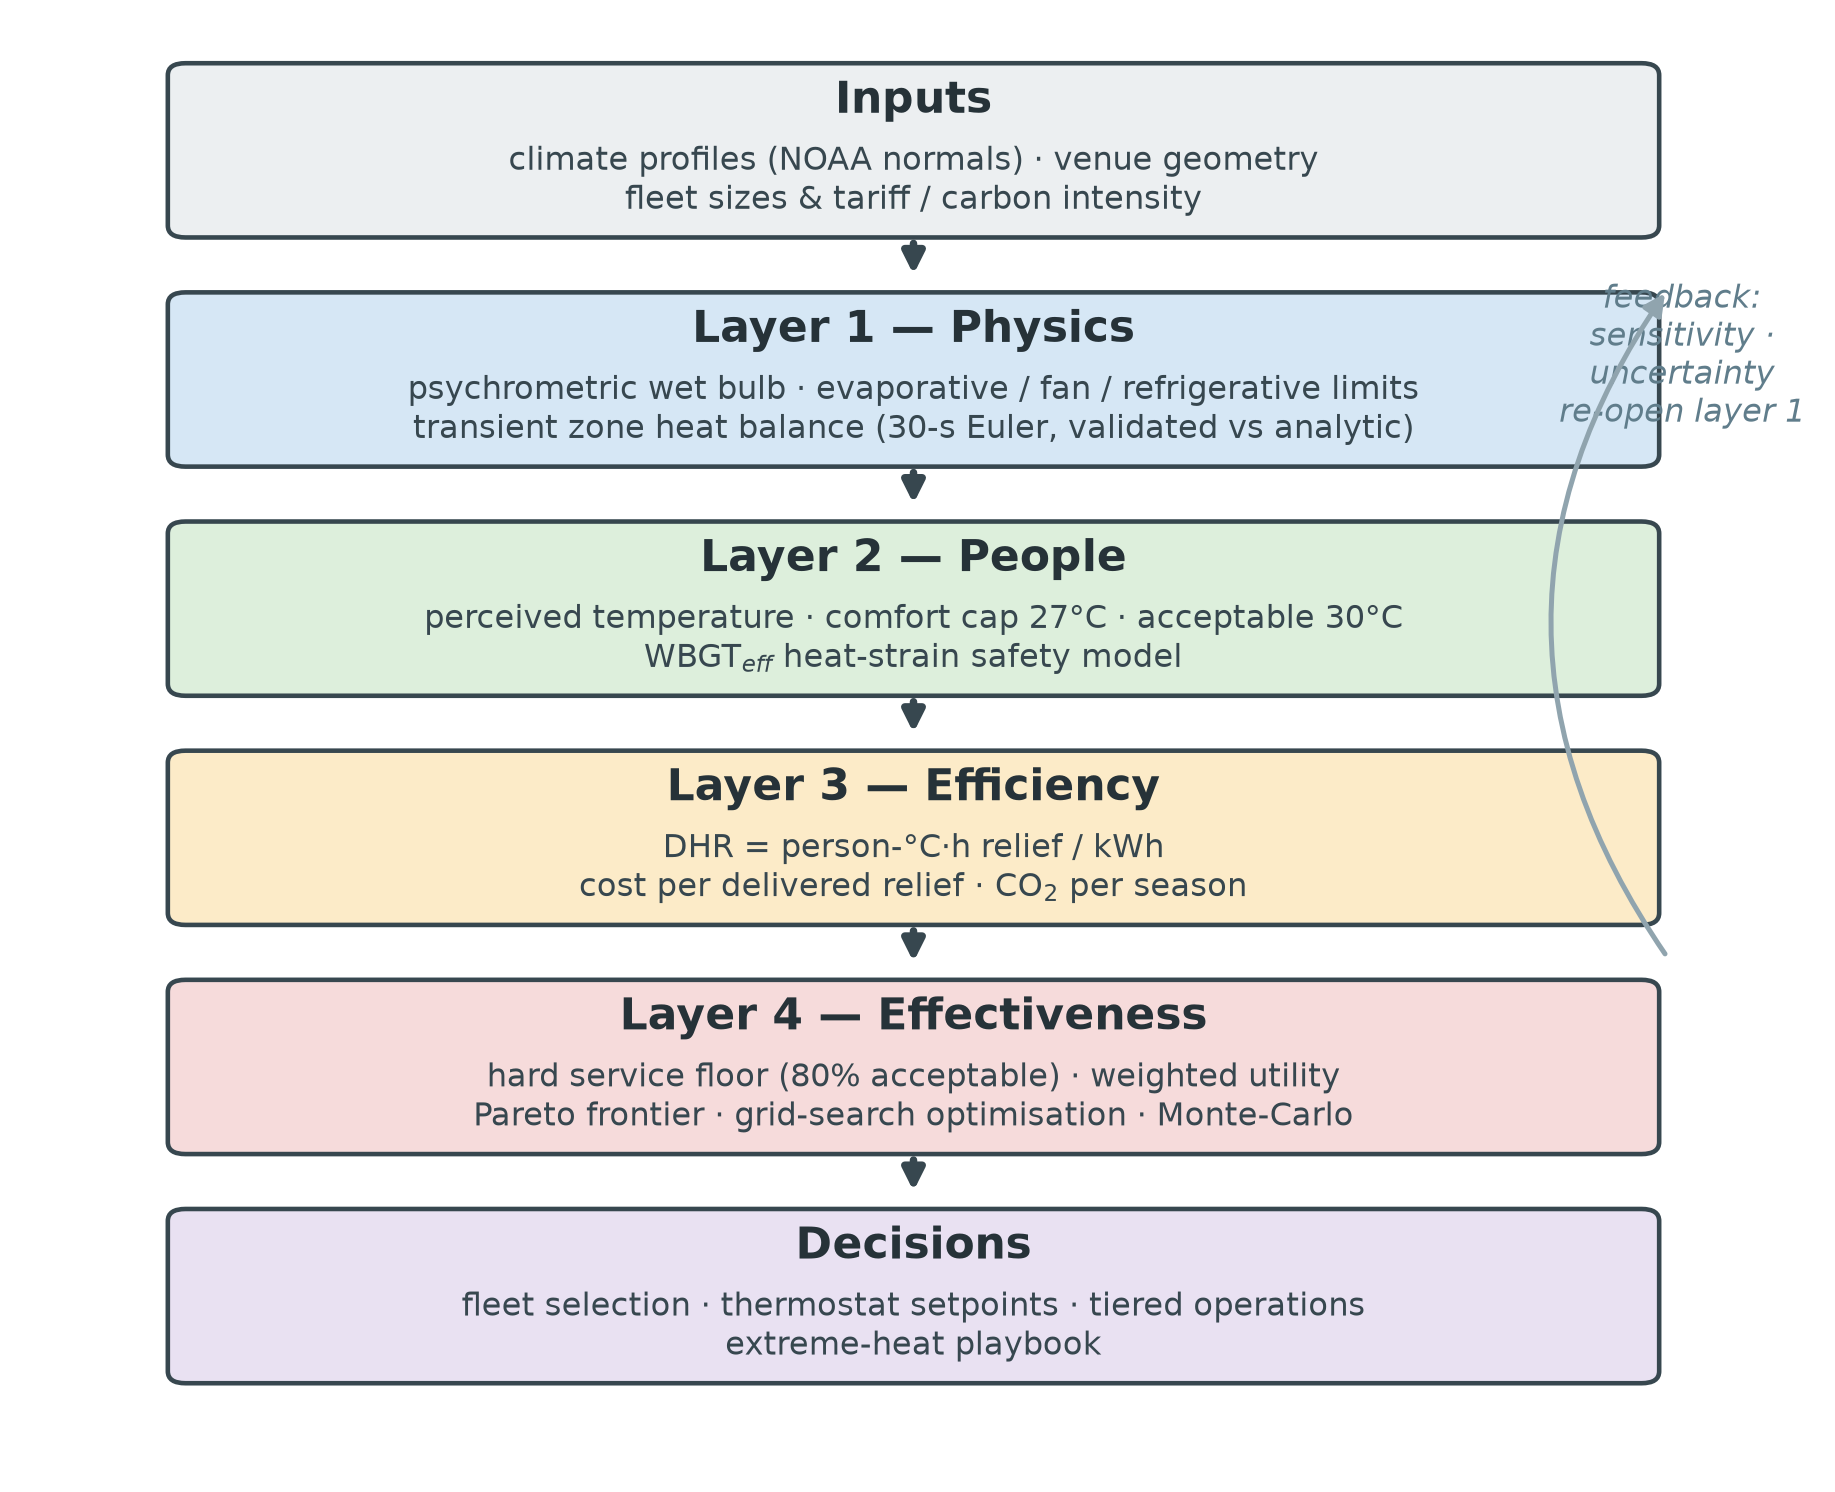
\includegraphics[width=0.72\linewidth]{fig0_framework.png}
\caption{The modelling framework. Sensitivity, optimisation and uncertainty analyses feed back into the physics layer.}\label{fig:framework}
\end{figure}

%=====================================================================
\section{Understanding the Problem: What the Freezer Case Teaches (Req.\ 1)}
%=====================================================================
\subsection{The freezer case as a control volume}
An open freezer case keeps food cold while its front face stands open to a warm sales floor. Drawing a control volume around the case (Fig.~\ref{fig:cv}), three fluxes matter: heat removed by the refrigeration plant ($E_{\text{in}}$ converted to thermal effect), heat leaking in through the open boundary (air exchange, convection, radiation), and the \emph{useful} fraction that actually reaches the product and the shopping aisle air. Industry practice reflects this decomposition: night curtains and air curtains raise efficiency precisely by shrinking the loss term, not by adding cooling power --- and the penalty for ignoring it is quantified by field audits, which find open cases consume roughly 30\% more energy than closed-door equivalents \cite{greenchill}.

\begin{figure}[H]\centering
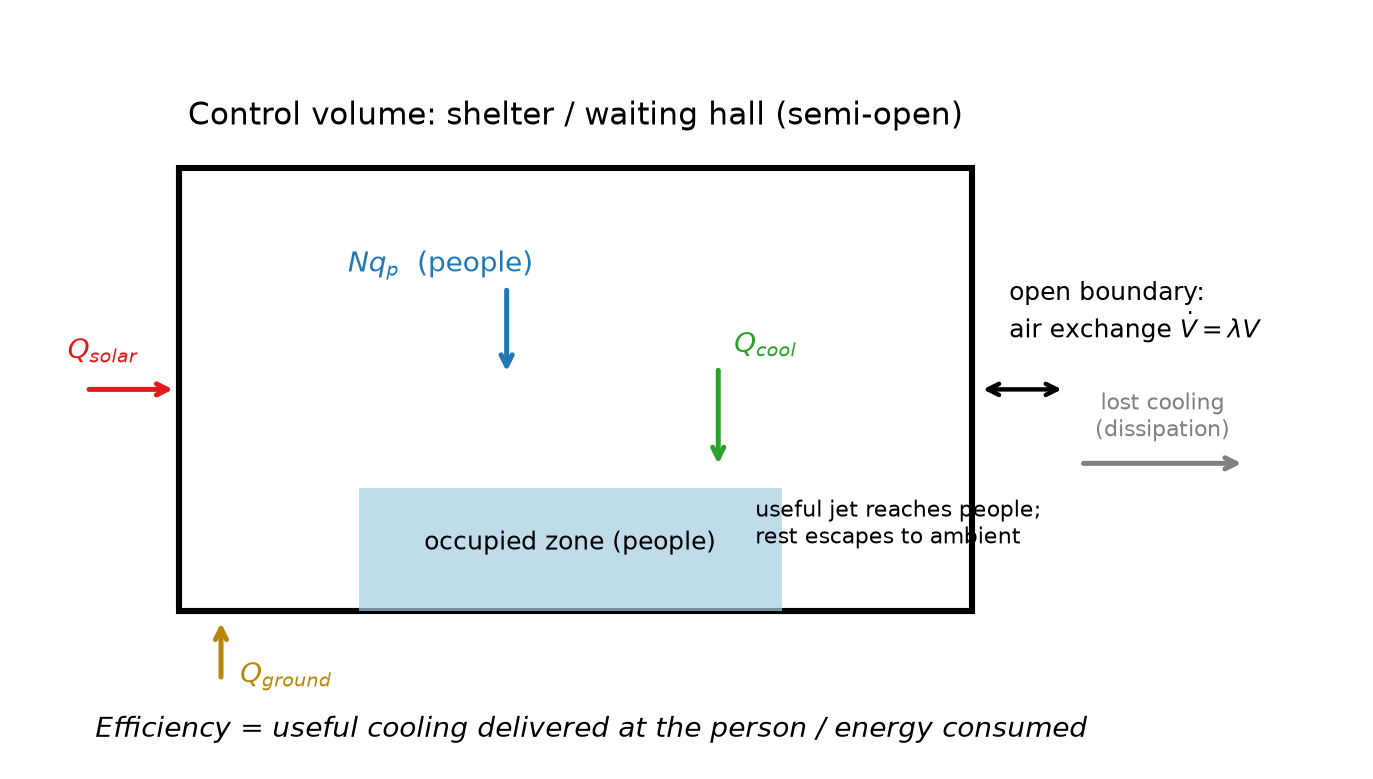
\includegraphics[width=0.88\linewidth]{fig1_control_volume.png}
\caption{Control volume for a semi-open cooled space. Only the cooling that reaches the occupied zone is useful; the rest dissipates to ambient. The same accounting applies to a freezer case, a bus shelter, or a rail hall.}
\label{fig:cv}
\end{figure}

\subsection{Why efficiency cannot depend on energy use alone}
Three thought experiments show why ``energy in'' is insufficient:
\begin{itemize}
\item A system that consumes nothing achieves a perfect ratio of anything-to-energy while cooling nobody; energy-only metrics reward doing nothing.
\item Two systems with equal kWh can deliver wildly different service depending on climate: an evaporative cooler that promises $8\degrees$C of drop in Phoenix delivers less than $6\degrees$C in Singapore --- and only $4.5\degrees$C of felt relief once the comfort cap is applied.
\item A system can be individually efficient yet collectively useless: in an open shelter, air exchange exceeds hundreds of volumes per hour, so a 1.2~kW cooler changes the \emph{room} temperature by well under $1\degrees$C while still helping the person standing in its jet.
\end{itemize}
Efficiency is therefore a property of \emph{service delivered}, measured where the person is.

\subsection{Quantities that belong in a measure of cooling efficiency}
\begin{enumerate}[label=\textbf{Q\arabic*.}]
\item \textbf{Useful cooling delivered} --- the accumulated relief experienced by people (person-$\degrees$C$\cdot$h), not thermal tons generated at the duct.
\item \textbf{Energy consumed} (kWh) and its \textbf{cost} (\$), the denominator resources actually paid.
\item \textbf{Beneficiaries and coverage} --- how many people are inside the cooled footprint; cooling an empty corner is waste.
\item \textbf{Climate conditions} --- wet-bulb depression (for evaporative systems), humidity (for fans), wind and enclosure fraction (for losses).
\item \textbf{Quality of service} --- comfort (fraction of time in the acceptable band) and \emph{safety} (heat-strain exposure), because a barely-cooled crowd can still be a casualty statistic.
\end{enumerate}
These five families motivate the design of our models: a service-based numerator, energy and money denominators, climate-adjusted achievable effects, and a safety layer imposed as a hard constraint on top of efficiency (Sec.~6).

%=====================================================================
\section{Assumptions, Justifications, and Notation}
%=====================================================================
\begin{enumerate}[label=\textbf{A\arabic*.}]
\item The problem's ``kW/hr'' entries are read as electrical power while operating: 0.25~kW means 0.25~kWh per operating hour. \textit{Justification:} kW/hr is not a physical unit of consumption; the table's intent is clearly hourly energy.
\item Evaporative systems operate at saturation effectiveness $\eta=0.85$ and can never exceed their rated drop: $\Delta T_e=\min(\Delta T_{\text{rated}},\ \eta\,(T_{db}-T_{wb}))$. \textit{Justification:} standard evaporative-cooler engineering limits \cite{ashrae}; the word ``up to'' in the problem.
\item A fan's rated ``feels $3\degrees$C cooler'' is a perceived-temperature offset for people inside its footprint, scaled by humidity: benefit is full below 40\% RH and decays linearly to 30\% at saturation (sweat evaporation is suppressed in humid air). \textit{Justification:} air-motion comfort literature; ASHRAE 55 elevated-air-speed provisions \cite{ashrae55}.
\item A waiting person contributes $\approx$55--75~W sensible heat (light activity); cooling an unoccupied hour is worth nothing.
\item Comfort cap: relief is valued only down to a perceived $27\degrees$C (cooler than that, nobody needs more); ``acceptable'' is perceived $\leq 30\degrees$C and WBGT$_{\text{eff}}\leq32\degrees$C; heat strain is perceived $>38\degrees$C or WBGT$_{\text{eff}}>32\degrees$C \cite{acgih,sherwood,epa}. Shaded-globe offset $1.5\degrees$C.
\item Spot-cooling footprints (bus stop): fan 6~m$^2$ (benches), evaporative 12~m$^2$, large evaporative 22~m$^2$; 0.75~m$^2$ per waiting person.
\item Semi-open hall ($40\times12\times4$~m): air exchange $\lambda = 3 + 2v$ ACH ($v$ = wind, m/s); envelope $UA=180$~W/K; solar gain through the open front up to 4~kW; effective thermal mass 4 air-volumes (structure included).
\item Train timetable: arrivals every 12 min at peaks (7--9h, 17--19h) and 20 min otherwise; each arrival adds a pulse of $\approx$70 passengers decaying in $\tau=4$~min (platform clearing), occupancy capped at 140.
\item Electricity at \$0.14/kWh; capital costs: fan \$250, evaporative \$900, large evaporative \$2200 (bus stop, 6-year life); station fleets \$10k (evaporative) / \$7k (refrigerative) over 7 years.
\item Indoor wet-bulb shift: occupants add $\approx+0.4$~K; evaporative operation a further $\approx+0.2$~K; refrigerative units dehumidify ($-1.4$~K). \textit{Justification:} mass balance at the high air-exchange rates of a semi-open hall.
\end{enumerate}

\begin{table}[H]\centering\small
\caption{Notation.}\label{tab:notation}
\begin{tabular}{@{}llll@{}}
\toprule
Symbol & Meaning & Symbol & Meaning\\
\midrule
$T_{db},T_{wb}$ & dry-/wet-bulb temperature & $\lambda$ & air-exchange rate (ACH)\\
$RH$ & relative humidity & $G_v$ & ventilation conductance $\rho c_p\lambda V/3600$\\
$\Delta T_{\text{rated}}$ & rated temperature drop & $C$ & zone thermal capacity $\rho c_p V\kappa$\\
$\eta$ & evaporative saturation effectiveness & $Q_c$ & useful cooling power (W)\\
$r$ & effective relief per person ($\degrees$C) & $S(t)$ & solar gain (W)\\
$N$ & occupancy (persons) & $T_p$ & perceived temperature ($\degrees$C)\\
$A_c$ & cooled footprint (m$^2$) & $\DHR$ & person-$\degrees$C$\cdot$h relief per kWh\\
$P$ & electric power (kW) & $E^\ast$ & effectiveness score (0--1)\\
\bottomrule
\end{tabular}
\end{table}

\begin{table}[H]\centering\footnotesize
\caption{Parameter provenance: every quantitative anchor is tied to a standard, a field-audit programme, or a station record.}\label{tab:prov}
\begin{tabular}{@{}p{4.0cm}p{2.8cm}p{6.6cm}@{}}
\toprule
Parameter & Value used & Source / anchor\\
\midrule
Evaporative effectiveness $\eta$ & 0.85 & ASHRAE: 0.70--0.90 typical for well-maintained pads \cite{ashrae}\\
Fan benefit & 3$\degrees$C below $\approx$40\% RH & elevated-air-speed comfort provisions \cite{ashrae55}; problem statement\\
Sensible heat per person & 55--75 W & seated, light activity \cite{ashrae}\\
Envelope & $UA=180$ W/K; $\lambda=3+2v$ ACH & louvered semi-open envelope estimate (Monte-Carlo-tested $\pm$30--40\%)\\
Comfort set points & 27 / 30 / 38$\degrees$C & ASHRAE 55 comfort band; caution limits \cite{ashrae55,acgih}\\
WBGT limit & 32$\degrees$C & ACGIH TLV, light activity \cite{acgih}\\
Refrigerative COP & 3.2 & commercial split equipment 3--4 \cite{doe}\\
Electricity price & \$0.14/kWh & EIA U.S. commercial average \cite{eia}\\
Grid carbon intensity & 0.49--0.52 kg CO$_2$e/kWh & EPA eGRID subregional output rates \cite{epagrid}\\
Climate design days & Table~\ref{tab:bus} headers & July station normals: Phoenix 41$\degrees$C/20\%, Miami 32$\degrees$C/63\%, Honolulu 30$\degrees$C/52\% \cite{noaa}; Guangzhou 33$\degrees$C (afternoon RH $\approx$75\%)\\
Open-case penalty & $\approx$30\% & EPA GreenChill field audits \cite{greenchill}\\
\bottomrule
\end{tabular}
\end{table}

%=====================================================================
\section{Model I: The Open-Sided Bus Stop (Req.\ 2a)}
%=====================================================================
\subsection{Physics: what each system can actually achieve}
\textbf{Evaporative systems (B, C).} Cooling rate is capped by the wet-bulb depression, $T_{db}-T_{wb}$, solved from the psychrometric equation \cite{ashrae}
\begin{equation}
RH\; e_s(T_{db}) \;=\; e_s(T_{wb}) - \gamma\,(T_{db}-T_{wb})\,(1+0.00115\,T_{wb}),\qquad \gamma = 0.00066\,P_{\text{atm}},
\end{equation}
with Tetens saturation pressure $e_s(T)=0.6108\,\exp(17.27\,T/(T+237.3))$~kPa \cite{ashrae}, cross-checked against Stull's closed-form fit \cite{stull}. Hence
\begin{equation}
\Delta T_e \;=\; \min\!\big(\Delta T_{\text{rated}},\; \eta\,(T_{db}-T_{wb})\big).
\label{eq:evap}
\end{equation}
\textbf{Fan (A).} Air motion cools people (convection plus sweat evaporation), not air:
\begin{equation}
\Delta T_f \;=\; 3.0\cdot\Big[1-0.7\,\max\!\big(0,\tfrac{RH-0.4}{0.6}\big)\Big]\quad(\degrees\text{C perceived}).
\label{eq:fan}
\end{equation}
\textbf{Comfort cap.} Cooling nobody needs is not useful, so the relief credited to any system is
\begin{equation}
r \;=\; \min\!\big(\Delta T_{\text{sys}},\; \max(0,\; T_{\text{env}}-27\degrees\text{C})\big).
\label{eq:cap}
\end{equation}

\subsection{The efficiency metric: Degree-Hours of Relief per kWh}
An open shelter exchanges hundreds of air volumes per hour; \emph{bulk} air temperature is uncontrollable, so service must be counted at the person. With $N_{\text{served}}=\min(N,\ A_c/0.75)$ people inside the footprint,
\begin{equation}
\boxed{\;\DHR \;=\; \frac{N_{\text{served}}\cdot r}{P}\;}
\qquad\text{[person-$\degrees$C$\cdot$h per kWh]}
\label{eq:dhr}
\end{equation}
$\DHR$ directly implements Q1--Q3 of Sec.~2.3: useful delivered relief (numerator), energy (denominator), and coverage (through $N_{\text{served}}$). Climate enters through Eqs.~(\ref{eq:evap})--(\ref{eq:cap}); safety enters as a separate flag (below), because averaging safety into a ratio would let dangerous-but-cheap systems buy a good score.

\subsection{Results}
\begin{table}[H]\centering\footnotesize
\caption{Bus-stop results at peak occupancy $N=12$ ($\DHR$ in person-$\degrees$C$\cdot$h/kWh; ``safe'' = served person below strain thresholds).}\label{tab:bus}
\begin{tabular}{@{}llrrrrrr@{}}
\toprule
Climate & System & $\Delta T$ (\degrees C) & served & $r$ (\degrees C) & $T_p$ (\degrees C) & $\DHR$ & safe\\
\midrule
%%TABLE_BUS%%
\bottomrule
\end{tabular}
\end{table}

Table~\ref{tab:bus} and Fig.~\ref{fig:bus} carry the punchline. In every climate the fan dominates $\DHR$ --- 96 person-$\degrees$C$\cdot$h/kWh in Phoenix against 50 (B) and 38.4 (C) --- because 0.25~kW buys a genuine $3\degrees$C of felt relief. Evaporative systems are clawed back by the wet bulb: at Miami's July normals ($32\degrees$C/63\%) both B and C sit within $0.05\degrees$C of the same wet-bulb-limited $4.95\degrees$C (Eq.~\ref{eq:evap}), so the cheaper B beats C at 49.5 vs.\ 23.8. In mild Honolulu the comfort cap Eq.~(\ref{eq:cap}) binds for the evaporative systems while the fan is throttled by humidity (Eq.~\ref{eq:fan}): at $30\degrees$C ambient only $3\degrees$C of relief is worth buying, again favouring the cheap fan. The complete 36-combination table is given in Appendix~A.

\begin{figure}[H]\centering
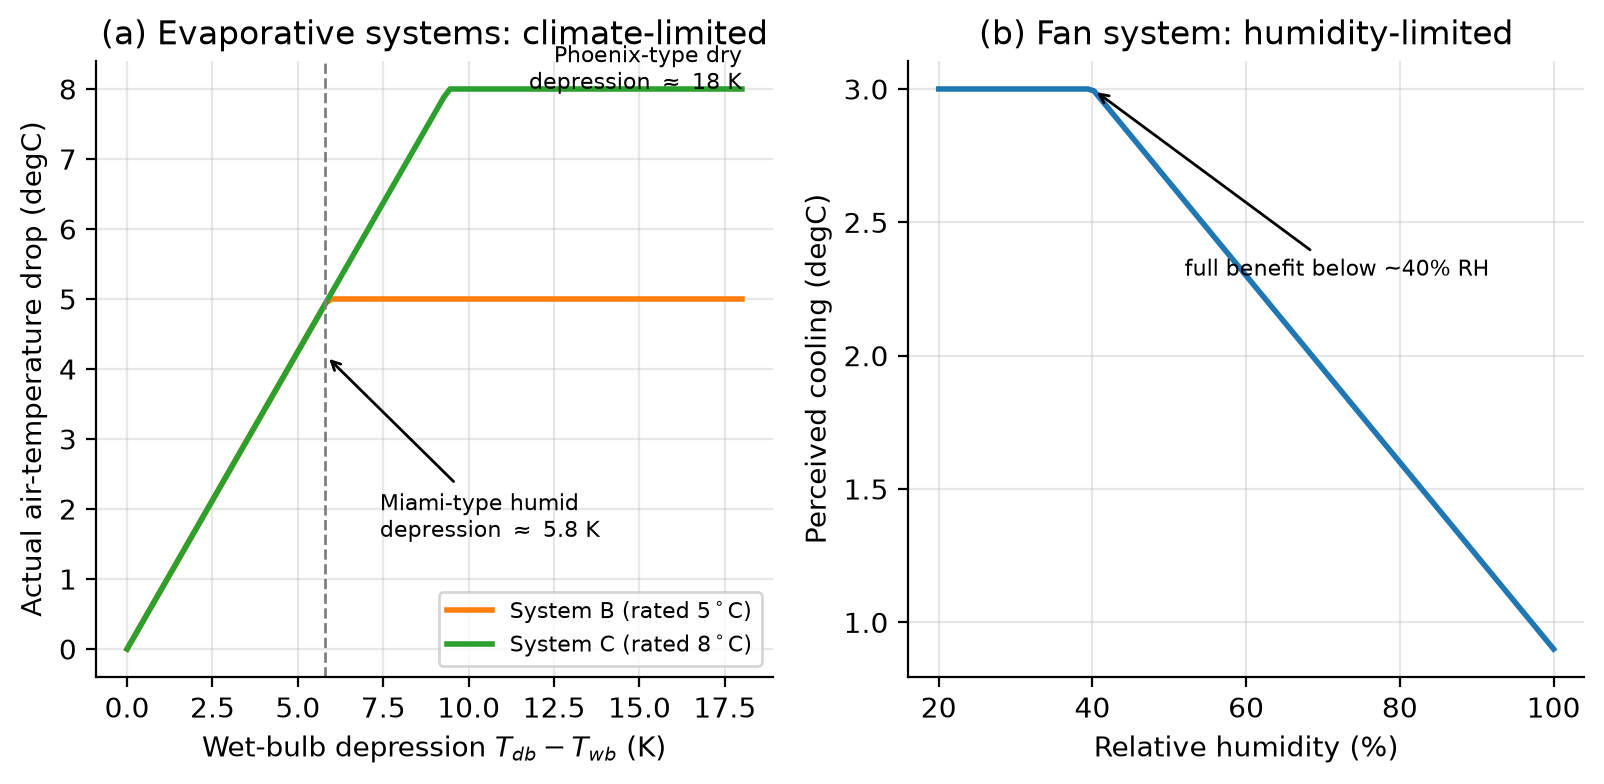
\includegraphics[width=0.98\linewidth]{fig2_system_response.png}
\caption{Climate limits. (a) Evaporative drop saturates at the rated value and collapses when the wet-bulb depression is small. (b) Fan benefit decays with humidity.}\label{fig:resp}
\end{figure}

\begin{figure}[H]\centering
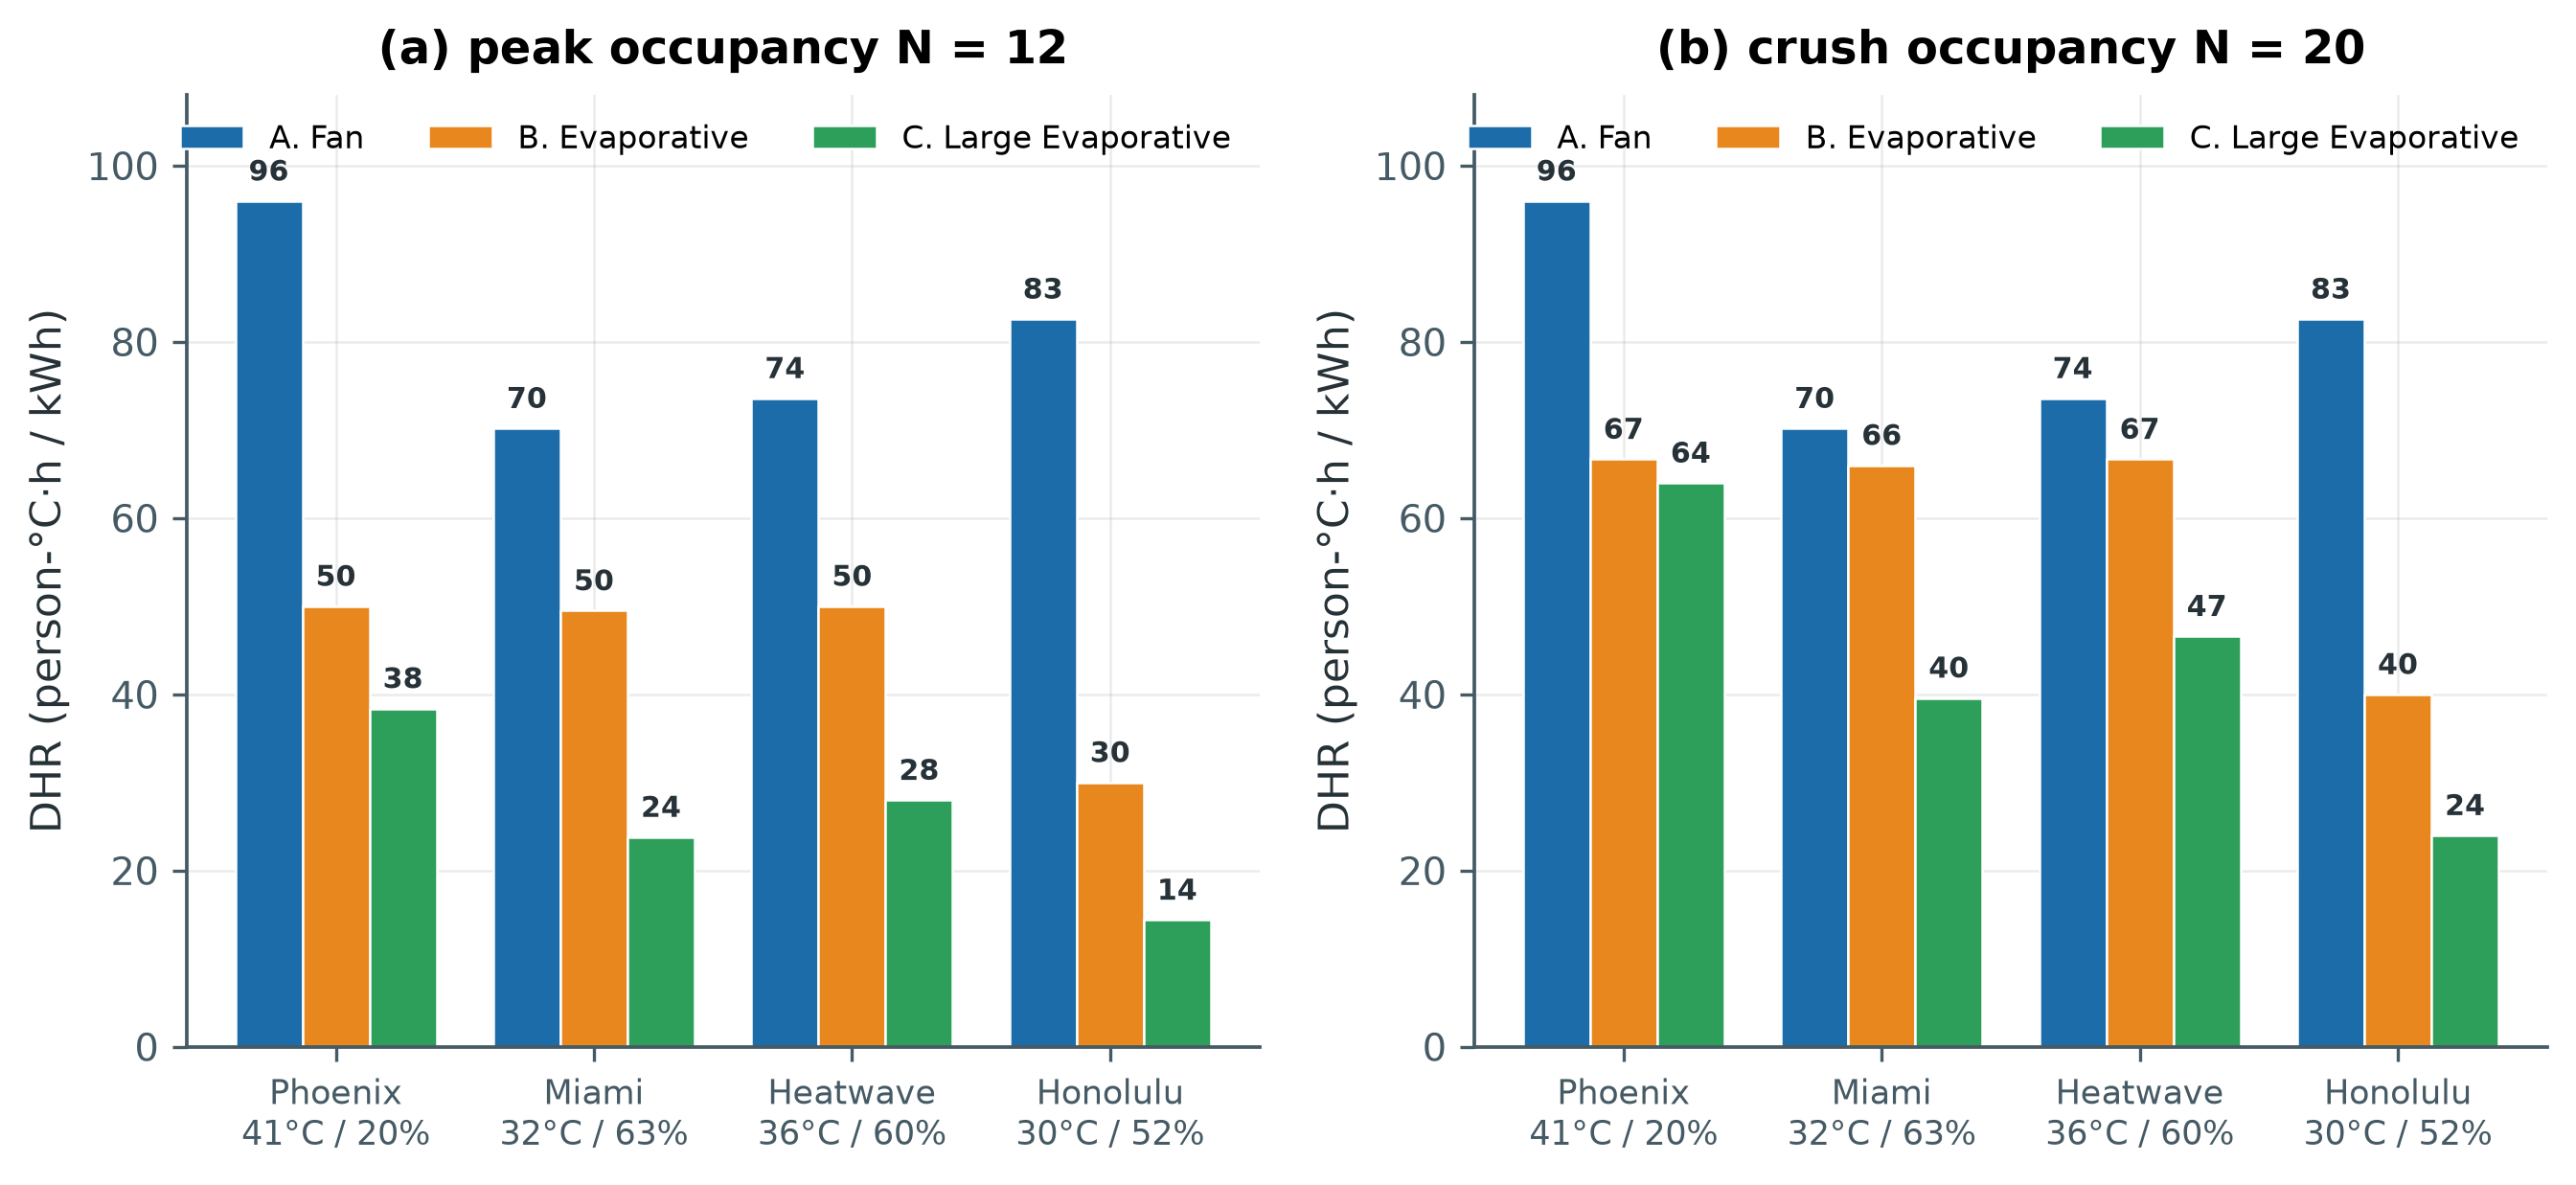
\includegraphics[width=0.98\linewidth]{fig3_bus_DHR.png}
\caption{$\DHR$ by climate and occupancy. Higher occupancy improves the evaporative systems' relative standing (more people share the bigger footprints) but never overtakes the fan on efficiency.}\label{fig:bus}
\end{figure}

\subsection{Cross-check: the thermodynamic view}
Counting thermal kW at the duct instead of felt relief at the person reverses the ranking --- evaporative units move 4.2 (B) and 6.4 (C) thermal-kW per electric-kW (a ``COP'' inflated by free water evaporation), versus $\approx$1.3 for fans. The metric choice \emph{is} the modelling decision: duct-kW rewards big machines; person-relief rewards cheap, well-placed ones. We report both, and justify $\DHR$ as primary because the brief asks for efficiency ``benefiting people'' (Req.~2a).

\subsection{Finding: the efficiency champion fails the safety bar}
At $41\degrees$C the fan leaves a served person at a perceived $38.0\degrees$C --- at the heat-strain threshold --- while the large cooler delivers $33\degrees$C. \emph{Efficiency and safety rank systems differently}, which is exactly why Req.~4 forces an effectiveness layer (Sec.~6), where rankings are computed under a hard safety floor --- and where the winning \emph{policy} (Sec.~5) pairs cheap baseline tiers with strong cooling under thermostat control.

%=====================================================================
\section{Model II: The Semi-Open Rail Station (Req.\ 2b)}
%=====================================================================
\subsection{What changed, why, and what it buys}
\begin{table}[H]\centering\small
\caption{Model revisions for the semi-open station and their justification.}\label{tab:rev}
\begin{tabular}{@{}p{3.4cm}p{4.6cm}p{6.6cm}@{}}
\toprule
Change & Why necessary & Improvement\\
\midrule
Steady-state $\to$ transient heat balance & A hall of 1920~m$^3$ has $\approx$38-min thermal time constant; occupant surges last 4--12 min. & Captures pre-cooling (the single largest operational saving); steady state underestimates surge peaks.\\
Person-centric spot model $\to$ zonal energy balance & Partial enclosure ($\psi\approx0.6$) retains cooled air; $\lambda\approx6$ ACH makes \emph{zone} temperature meaningful, unlike the open shelter. & Enables equipment sizing (fleet of units) and enclosure-design questions the shelter model cannot ask.\\
Comfort only $\to$ comfort + WBGT safety & Crowds cannot leave; safety becomes a constraint at scale. & Separate heat-strain exposure metric drives tiered operating policies.\\
Static occupancy $\to$ timetable pulses $N(t)$ & Rail demand is spiky (train arrivals), unlike a bus stop. & Pre-cooling windows can be optimised against the timetable.\\
Energy only $\to$ energy + amortised capital & Real procurement compares fleets, not devices. & Cost per delivered relief makes cross-venue comparisons honest.\\
\bottomrule
\end{tabular}
\end{table}

\subsection{Governing equations}
With ventilation conductance $G_v=\rho c_p \lambda V/3600$ and zone capacity $C=\rho c_p V\kappa$ ($\kappa=4$ includes structure), the hall temperature obeys
\begin{equation}
C\,\frac{dT_{in}}{dt} \;=\; UA\,(T_{out}-T_{in}) + S(t) + N(t)\,q_p + G_v\,(T_{out}-T_{in}) \;-\; Q_c(t),
\label{eq:ode}
\end{equation}
integrated at 30-s steps from 06:00 to 22:00. Evaporative fleets deliver
$Q_c = n_u\,\rho c_p \dot V_u\,\Delta T_e\,f_{\text{recirc}}$ (four units, $\dot V_u=6000$~m$^3$/h, recirculation $f_{\text{recirc}}=0.8$); refrigerative units deliver $2\times12$~kW at $f_{\text{recirc}}=0.65$, COP 3.2. Perceived temperature and an effective WBGT \cite{acgih} are
\begin{equation}
T_p = T_{in} - \Delta T_{\text{fan}},\qquad
\text{WBGT}_{\text{eff}} = 0.7\,(T_{wb}^{in}+\delta_{\text{latent}}) + 0.3\,(T_p+1.5),
\end{equation}
and we track (i) \textbf{heat-strain exposure} $H=\int N\,[\max(0,\text{WBGT}_{\text{eff}}-32)+\max(0,T_p-38)]\,dt$ in person-$\degrees$C$\cdot$h, (ii) \textbf{acceptable share} of person-time ($T_p\leq30\degrees$C and WBGT$_{\text{eff}}\leq32$), (iii) relief vs.\ the uncooled baseline, and (iv) daily cost (energy + amortised capital).

\subsection{Numerical validation}
Two checks are run before the model is used. \textbf{Energy-balance closure:} under constant forcing ($T_{out}=38\degrees$C, $RH=15\%$, $N=25$, $S=3$~kW, fleet on), Eq.~(\ref{eq:ode}) admits the analytic equilibrium $T_{in}^{*}=T_{out}-(Q_c-S-Nq_p)/(UA+G_v)$; the simulation converges to it to within $10^{-3}\,\degrees$C. \textbf{Step-size convergence:} refining the Euler step from 120~s to 7.5~s moves daily energy by at most $0.5\%$ (Table~\ref{tab:valid}); the 30~s production step is retained.

\subsection{Operating policies}
P0: nothing. P1: ceiling fans always (0.6~kW). P2: four large evaporative units always on. P3 (\textit{our policy}): fans always; evaporative fleet on a thermostat with hysteresis --- ON when $T_p>30\degrees$C or crowds exceed 70, OFF when $T_p<27.5\degrees$C, plus pre-cooling windows before the morning/evening surges. P4: refrigerative always on.

\begin{table}[H]\centering\small
\caption{Euler step-size study (P3, hot-arid design day): energy is step-size insensitive to $\pm0.5\%$.}\label{tab:valid}
\begin{tabular}{@{}rrrr@{}}
\toprule
$\Delta t$ (s) & kWh/day & $\max T_{in}$ (\degrees C) & $|$dev$|$ from finest (kWh)\\
\midrule
%%TABLE_VALID%%
\bottomrule
\end{tabular}
\end{table}

\subsection{Results}
\begin{figure}[H]\centering
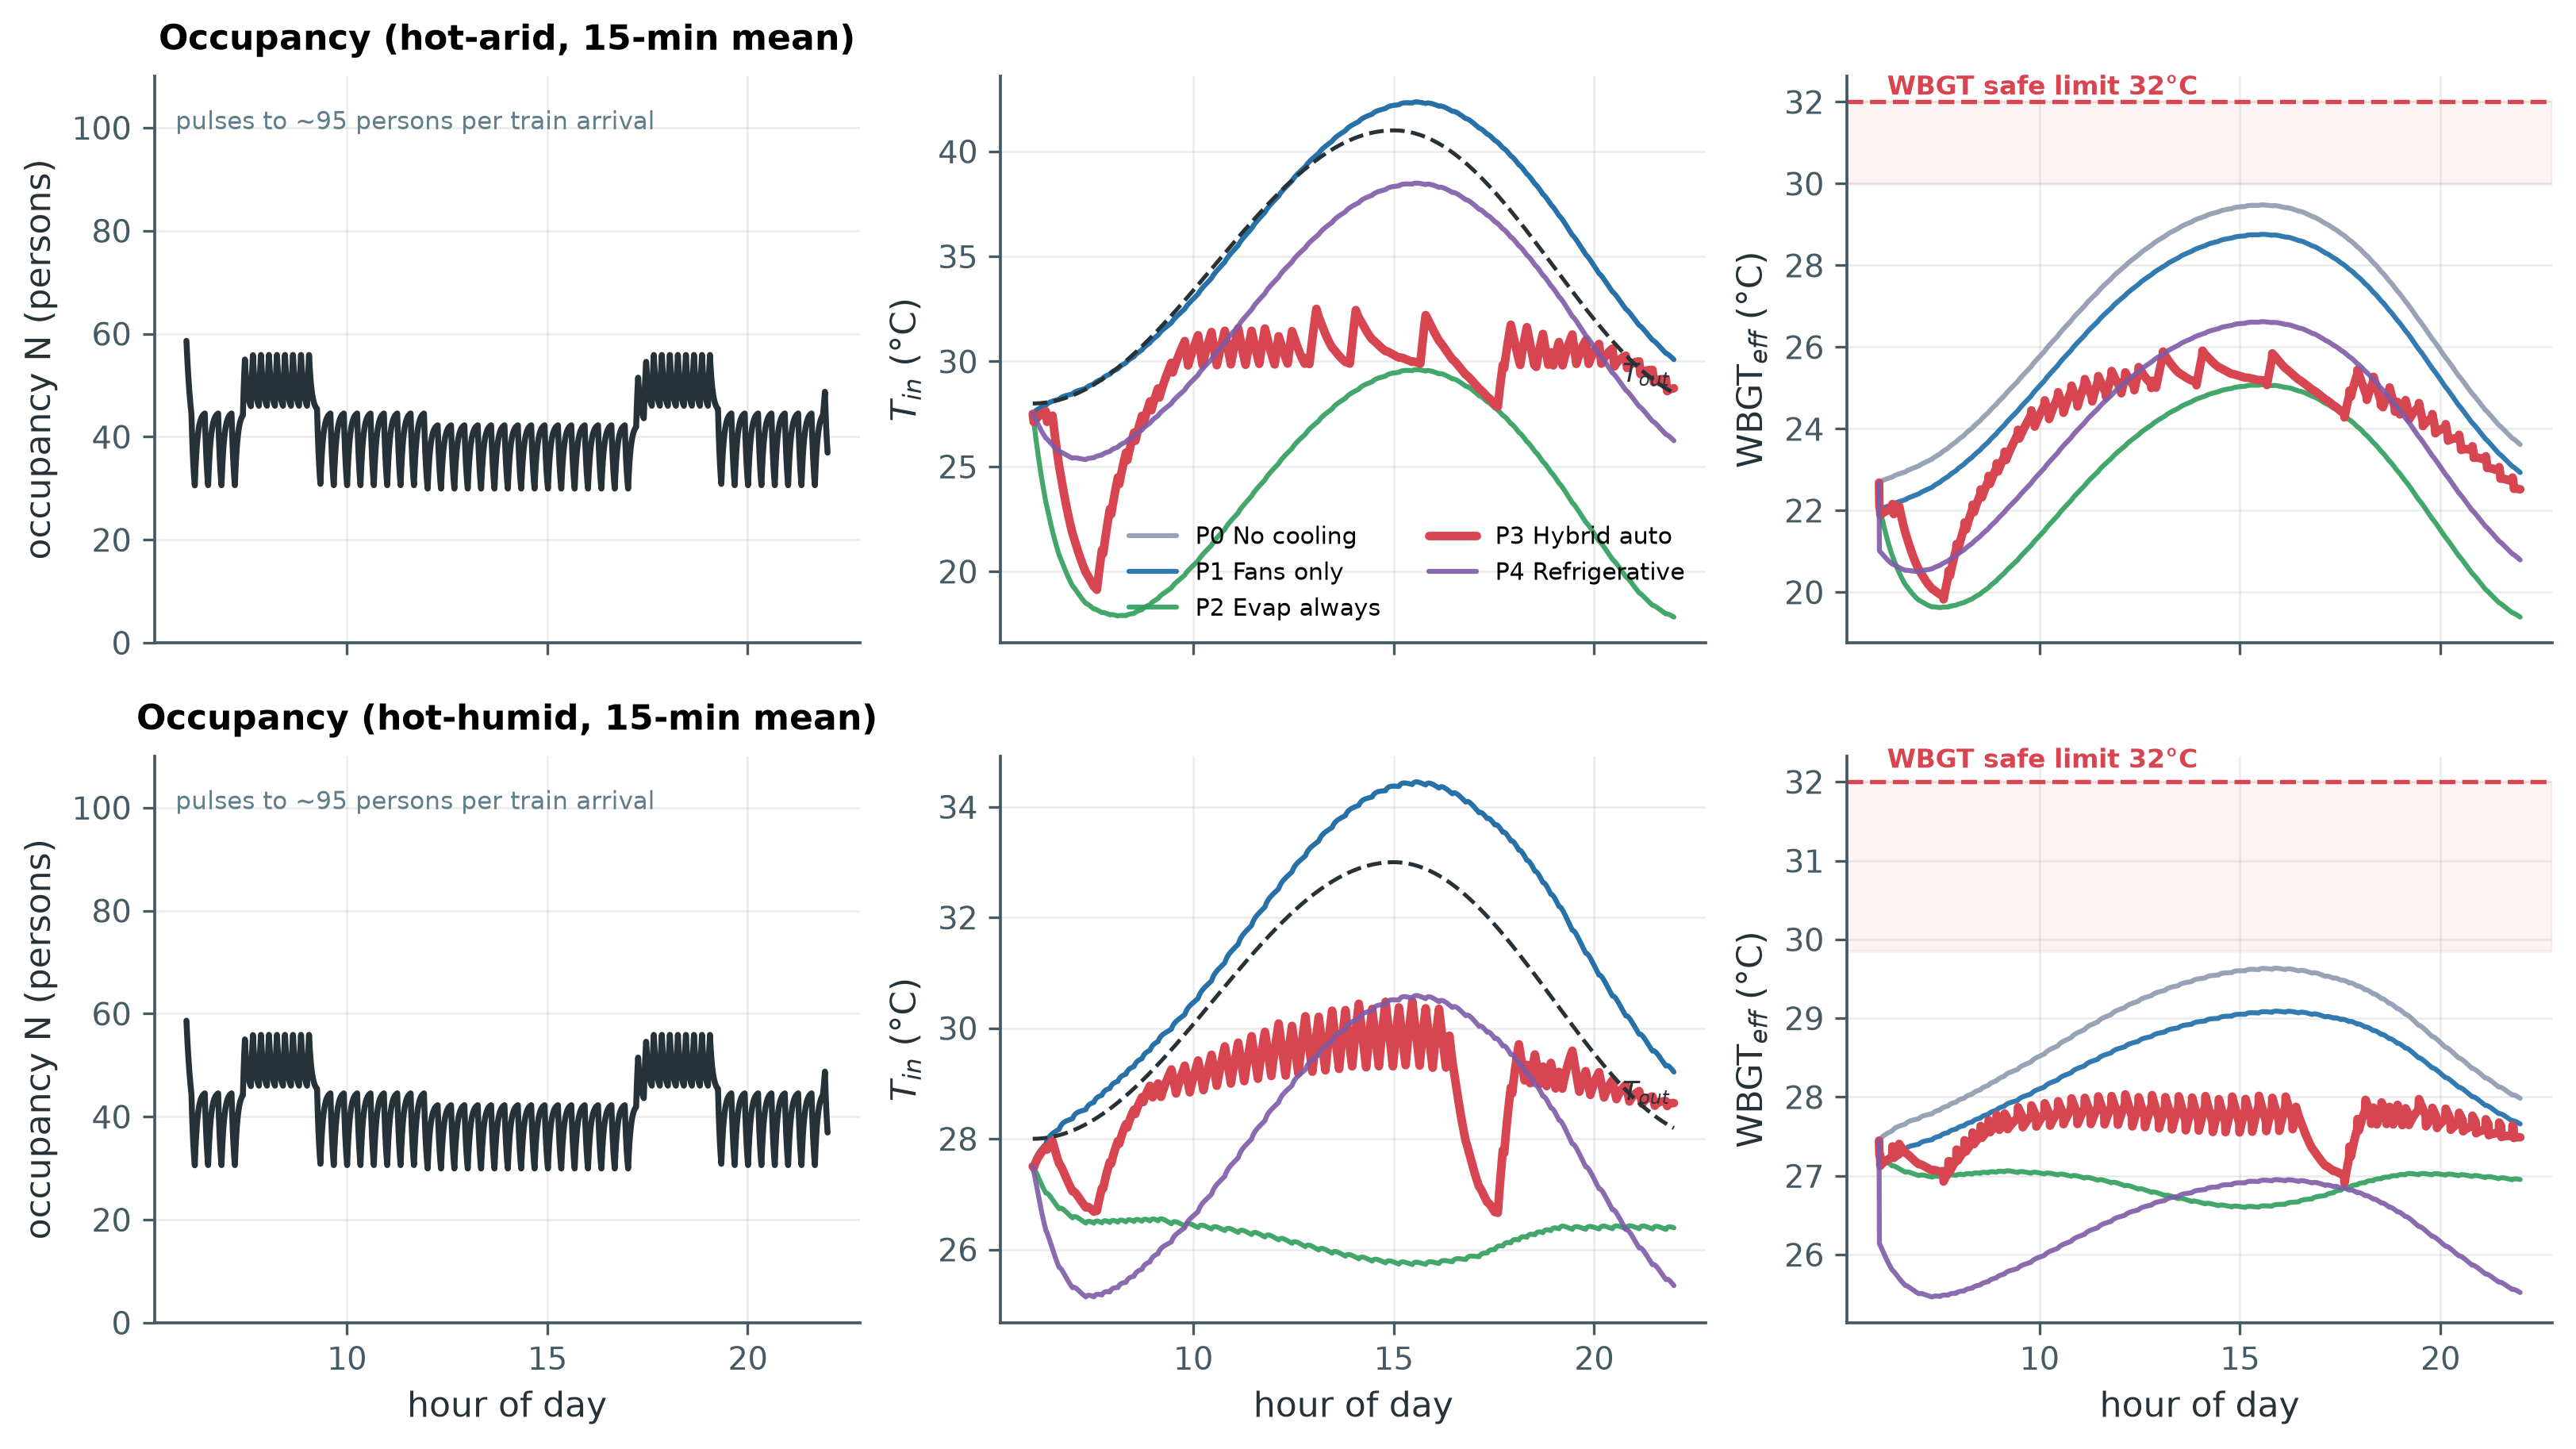
\includegraphics[width=0.99\linewidth]{fig4_station_timeseries.png}
\caption{Station simulation. Left: 15-min mean occupancy (pulses to $\approx$95 persons per arrival). Centre: hall temperature; the dashed black line is ambient. Right: effective WBGT against the 32$\degrees$C safe limit. The hybrid P3 tracks P2's comfort through the afternoon while using the plant half the time.}\label{fig:station}
\end{figure}

\begin{table}[H]\centering\small
\caption{Station policies (16-h operating day). ``ok'' = acceptable share of person-time; strain in person-$\degrees$C$\cdot$h; cost = energy + amortised capital.}\label{tab:station}
\begin{tabular}{@{}llrrrrrrr@{}}
\toprule
Climate & Policy & kWh/day & $\bar r$ (\degrees C) & $\DHR$ & strain & ok\,\% & \$/day & floor\\
\midrule
%%TABLE_STATION%%
\bottomrule
\end{tabular}
\end{table}

\begin{figure}[H]\centering
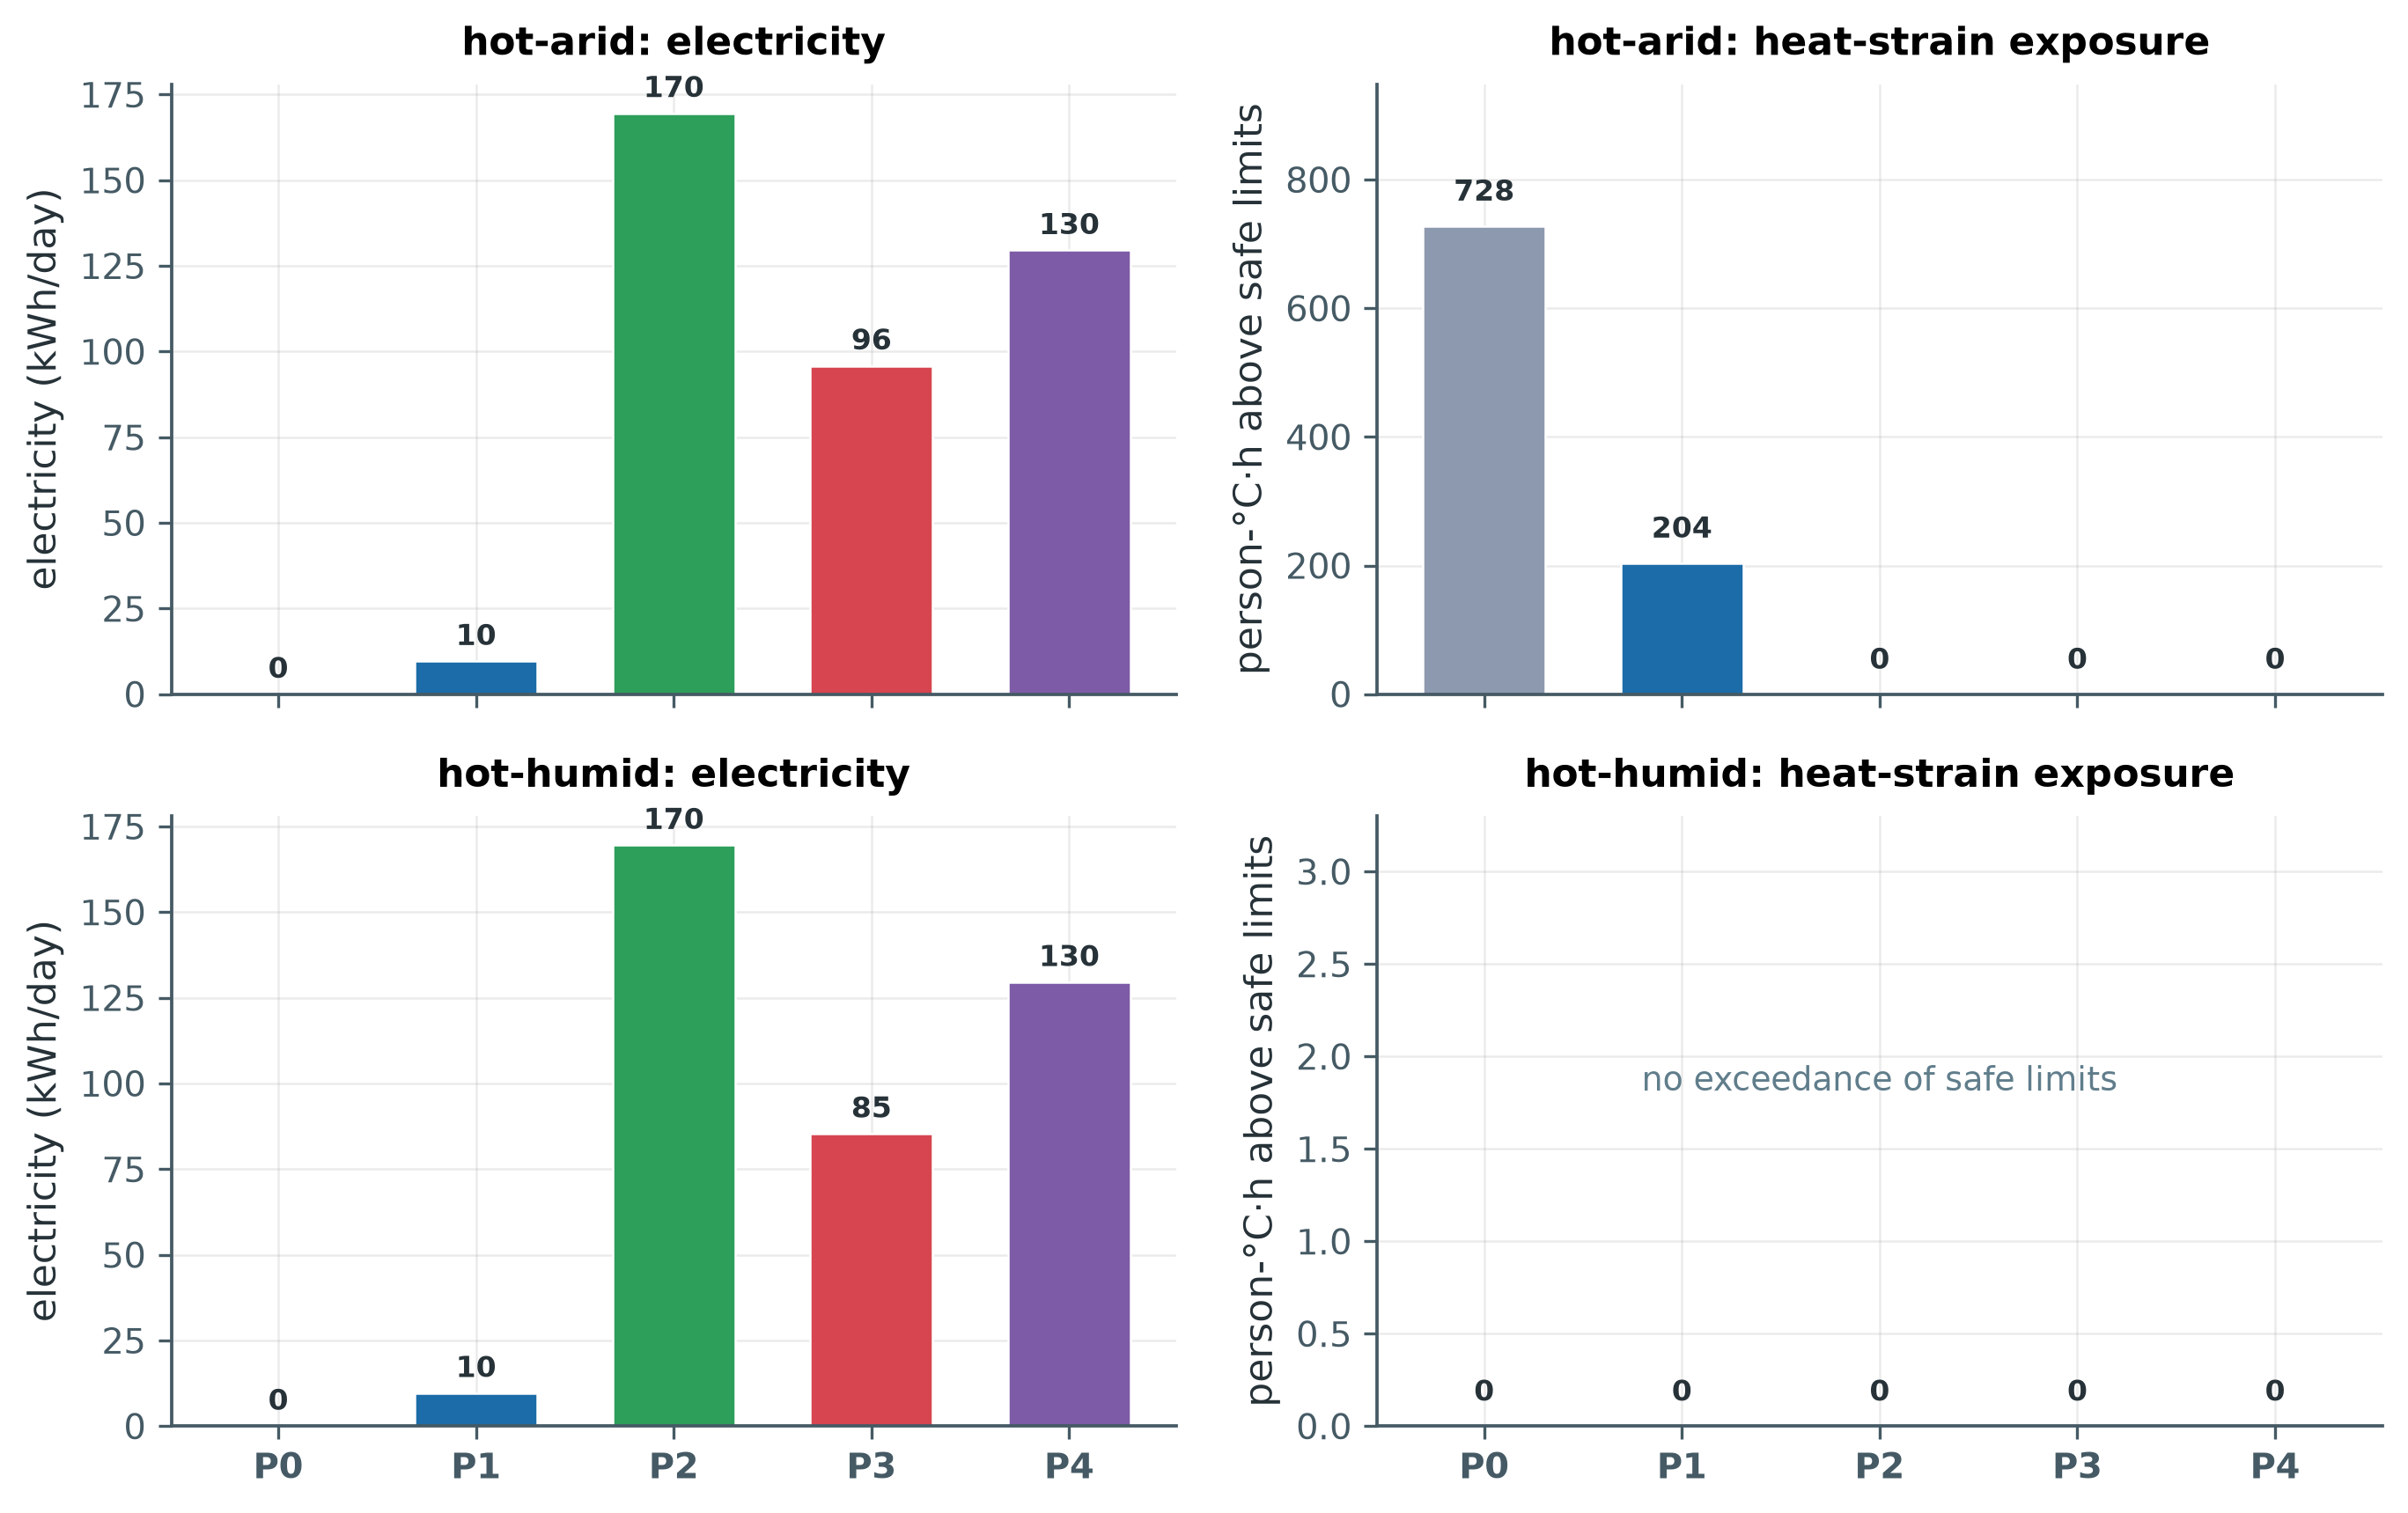
\includegraphics[width=0.96\linewidth]{fig5_policy_bars.png}
\caption{Energy vs.\ heat-strain exposure by policy. In hot-arid climates, doing nothing or fans-only leaves substantial heat-strain exposure (481 and 68 person-$\degrees$C$\cdot$h/day); every policy with real cooling eliminates it.}\label{fig:polbars}
\end{figure}

\textbf{Findings.} (1) In hot-arid heat, P2 holds the hall to $T_{in}\leq29.6\degrees$C but burns 169.5~kWh/day; P3 holds $\approx$100\% acceptable person-time at 95.8~kWh/day ($-$43.5\%) and cost \$18.9/day ($-$35\%). (2) In hot-humid heat, the evaporative fleet still works (afternoon RH $\approx60\%$ gives a 7.6~K depression) but refrigerative cooling becomes genuinely competitive: it dehumidifies, and at \$22.4/day it meets the floor that fans-only (46\% acceptable) fails. (3) The revised model surfaces an operational lever the shelter model could not even represent --- \emph{when} to run, not just \emph{what} to run.

\subsection{Optimising the thermostat: grid search and robust selection}
The nominal rule was not guessed: we grid-search $T_{on}\in[28.5,31]\degrees$C, hysteresis band $2$--$3.5\degrees$C and crowd trigger $N_{trig}\in\{70,90,\infty\}$ (72 designs per climate) under the constraints of the 80\% service floor and zero heat strain (Fig.~\ref{fig:opt}). On the nominal model, aggressive setpoints (e.g.\ $T_{on}=31\degrees$C, band 3$\degrees$C, no crowd trigger) cut energy a further 15--41\% below the nominal rule. Re-scoring every candidate under 150 Monte-Carlo plant draws, however, exposes them as fragile: the aggressive designs meet the service floor in only 52--85\% of draws, because they ride the floor with no margin. The \emph{robust} choice --- least energy subject to $P(\text{ok}\geq0.8)\geq95\%$ over the draws --- is precisely the nominal rule $(T_{on},\text{band},N_{trig})=(30\degrees\text{C},\,2.5\degrees\text{C},\,70)$ in both climates (Table~\ref{tab:robust}). The reliability premium is 15\% (arid) to 42\% (humid) of daily energy, and it is worth paying.

\begin{figure}[H]\centering
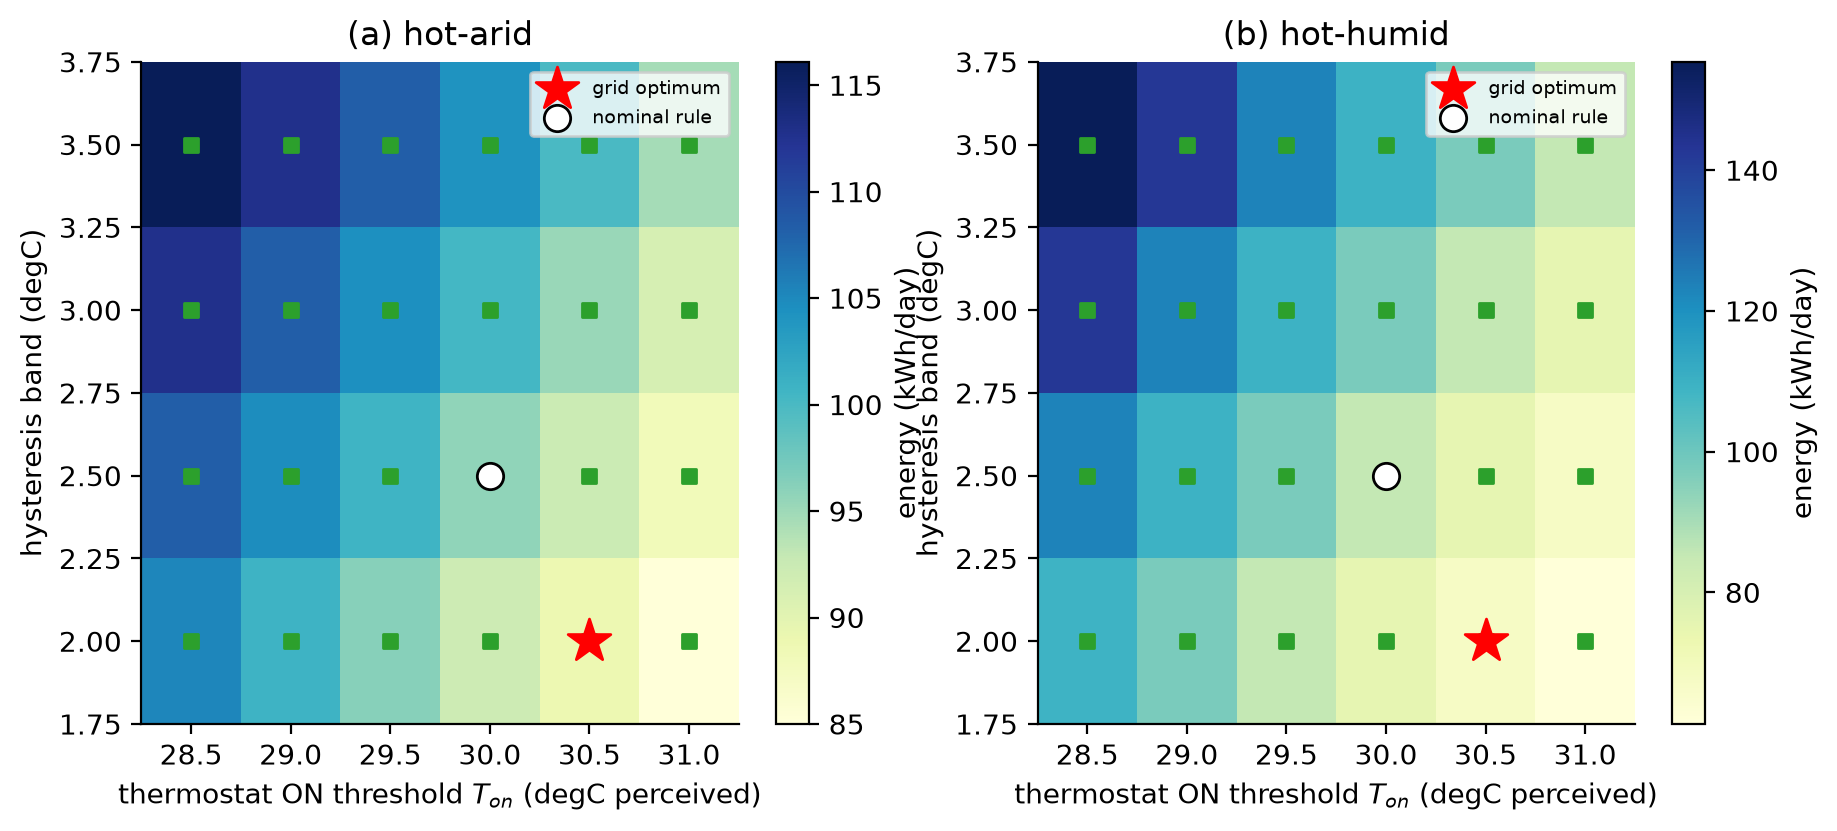
\includegraphics[width=0.98\linewidth]{fig10_opt_surface.png}
\caption{Thermostat grid search (crowd trigger $N=70$): daily energy over setpoint space; green squares mark nominal-model-feasible designs, the star the nominal-model optimum, the open circle the adopted rule.}\label{fig:opt}
\end{figure}

\begin{table}[H]\centering\small
\caption{Robust selection: leading candidates re-scored under 150 plant draws. $P_{\text{feas}}$: share of draws meeting the 80\% floor; bold = adopted robust optimum.}\label{tab:robust}
\begin{tabular}{@{}lrrrr@{}}
\toprule
Climate & $T_{on}$ / band / $N_{trig}$ & kWh (nominal) & $P_{\text{feas}}$ & ok P10\\
\midrule
%%TABLE_ROBUST%%
\bottomrule
\end{tabular}
\end{table}

%=====================================================================
\section{From Efficiency to Effectiveness (Req.\ 4)}
%=====================================================================
A cooling solution that is highly efficient may not be effective. We therefore impose a \textbf{hard service floor} --- at least 80\% of weighted person-time must be ``acceptable'' --- and, among feasible options, maximise a weighted utility
\begin{equation}
E^\ast \;=\; w_1\,\text{perf} + w_2\,\text{exp} + w_3\,\text{energy} + w_4\,\text{cost},
\qquad \mathbf{w}=(0.30,\,0.25,\,0.25,\,0.20),
\end{equation}
where perf = mean relief normalised by an $8\degrees$C reference, exp = acceptable person-time share, and energy/cost are min-max normalised within each comparison set.

\begin{table}[H]\centering\small
\caption{Effectiveness scores (bold = best feasible option in the panel; ``feasible'' = passes the 80\% service floor).}\label{tab:eff}
\begin{tabular}{@{}lllrrrrr@{}}
\toprule
Panel & Option & feasible & perf & exp & energy & cost & $E^\ast$\\
\midrule
%%TABLE_EFF%%
\bottomrule
\end{tabular}
\end{table}

\begin{figure}[H]\centering
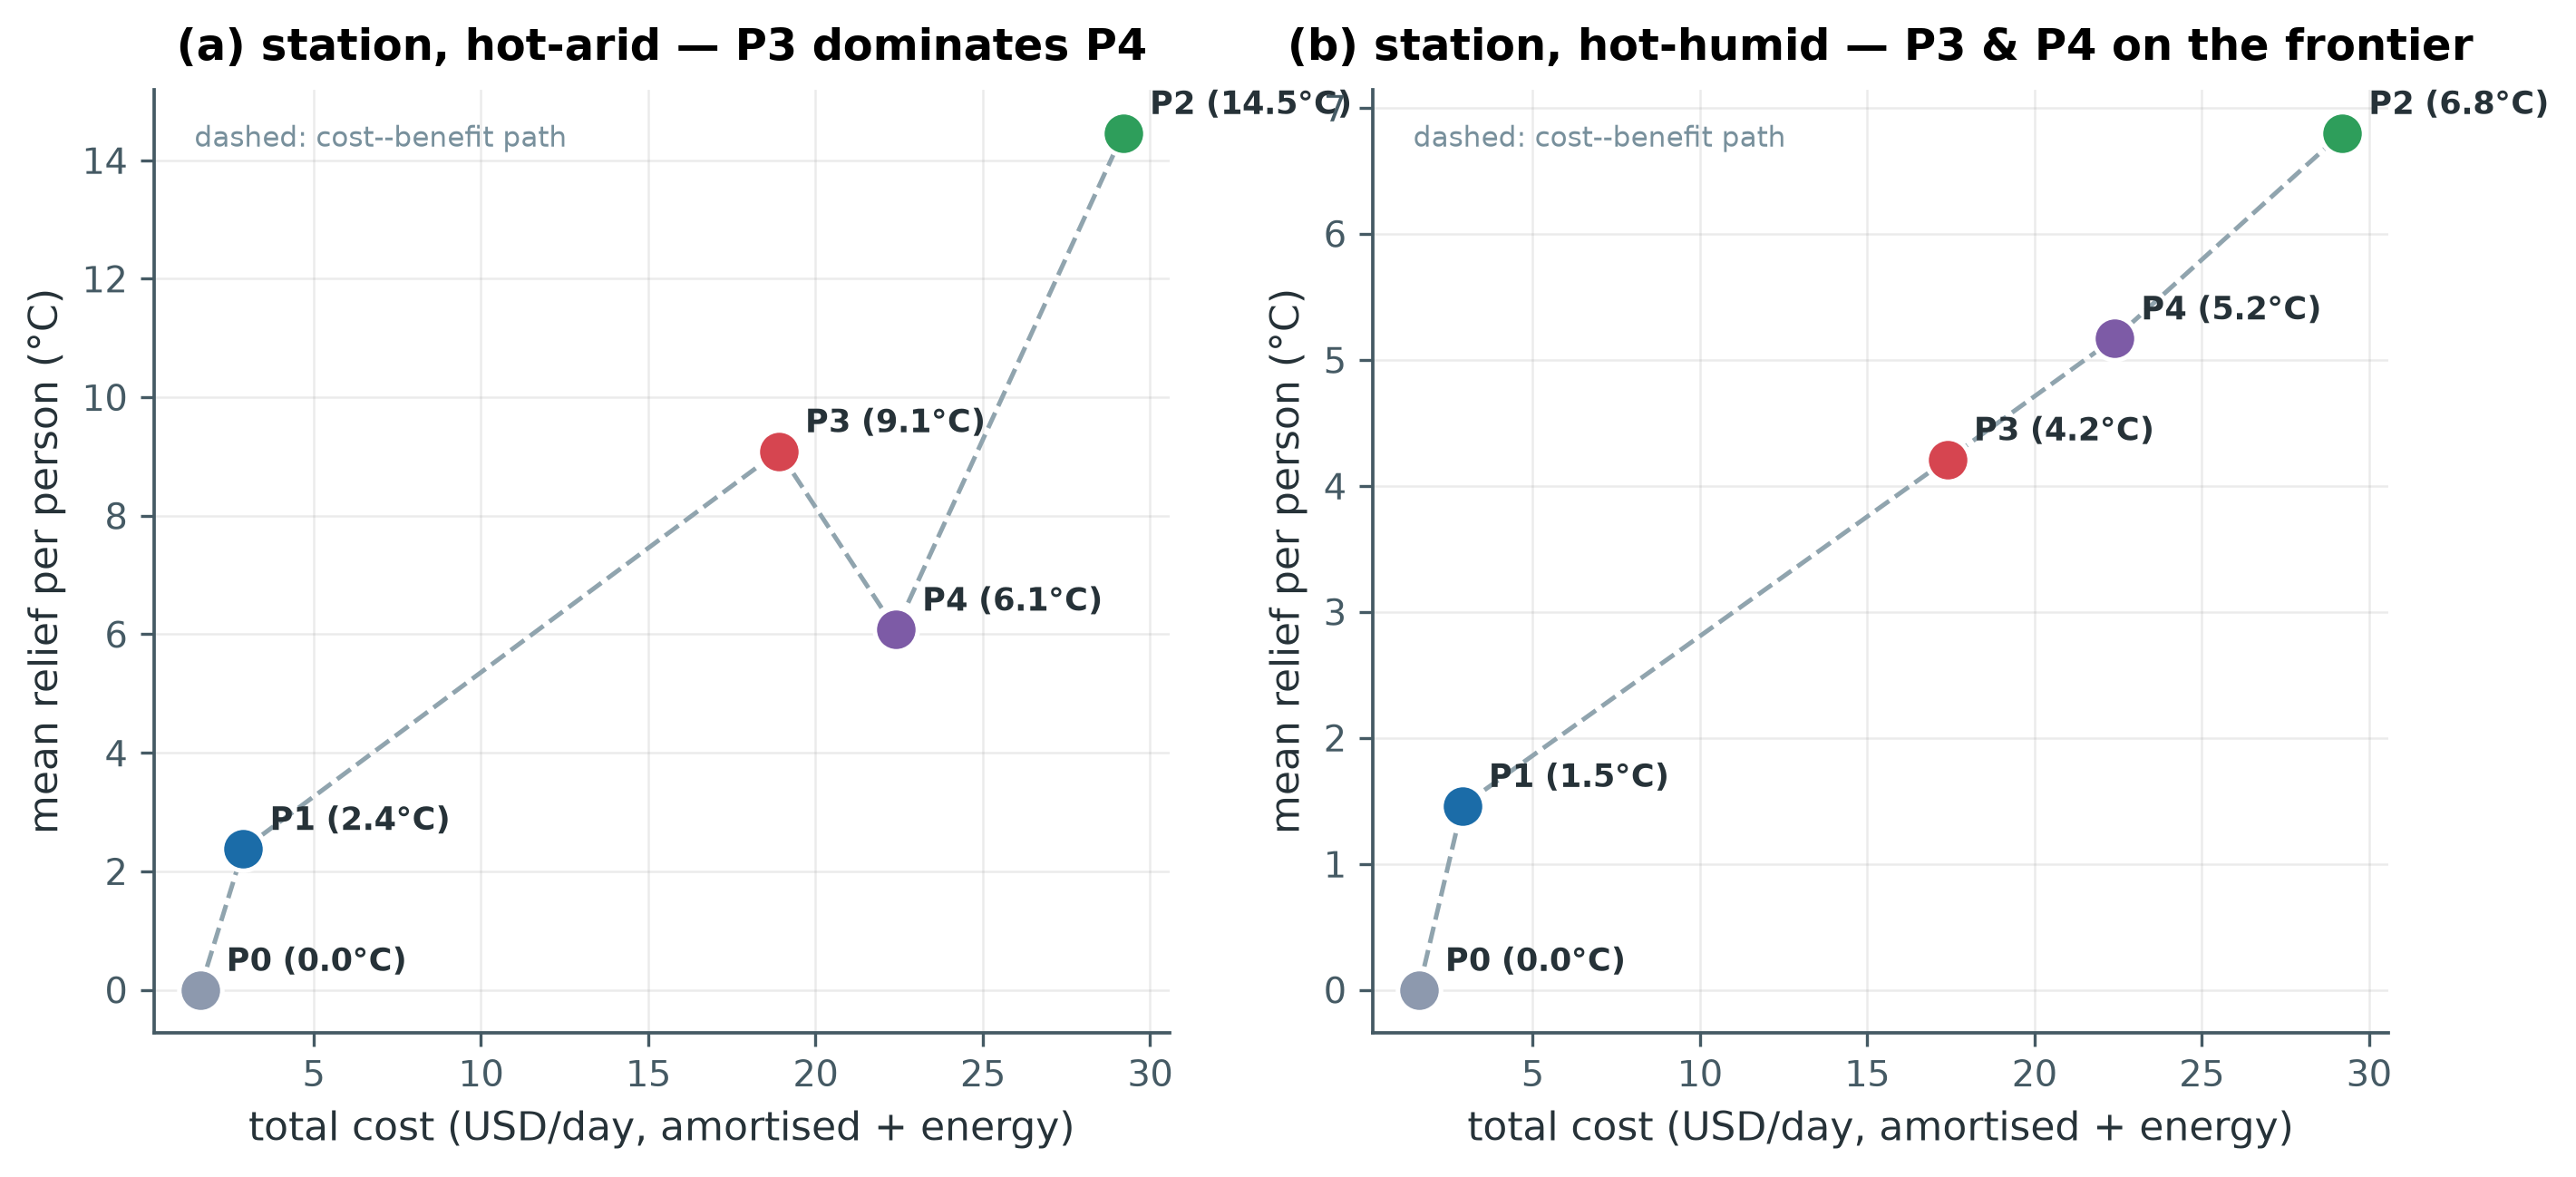
\includegraphics[width=0.97\linewidth]{fig7_pareto.png}
\caption{Cost--benefit frontier for station policies. In hot-arid climates P3 dominates P4 outright (more relief, less money); in hot-humid climates P3 and P4 sit on the frontier together.}\label{fig:pareto}
\end{figure}

\begin{figure}[H]\centering
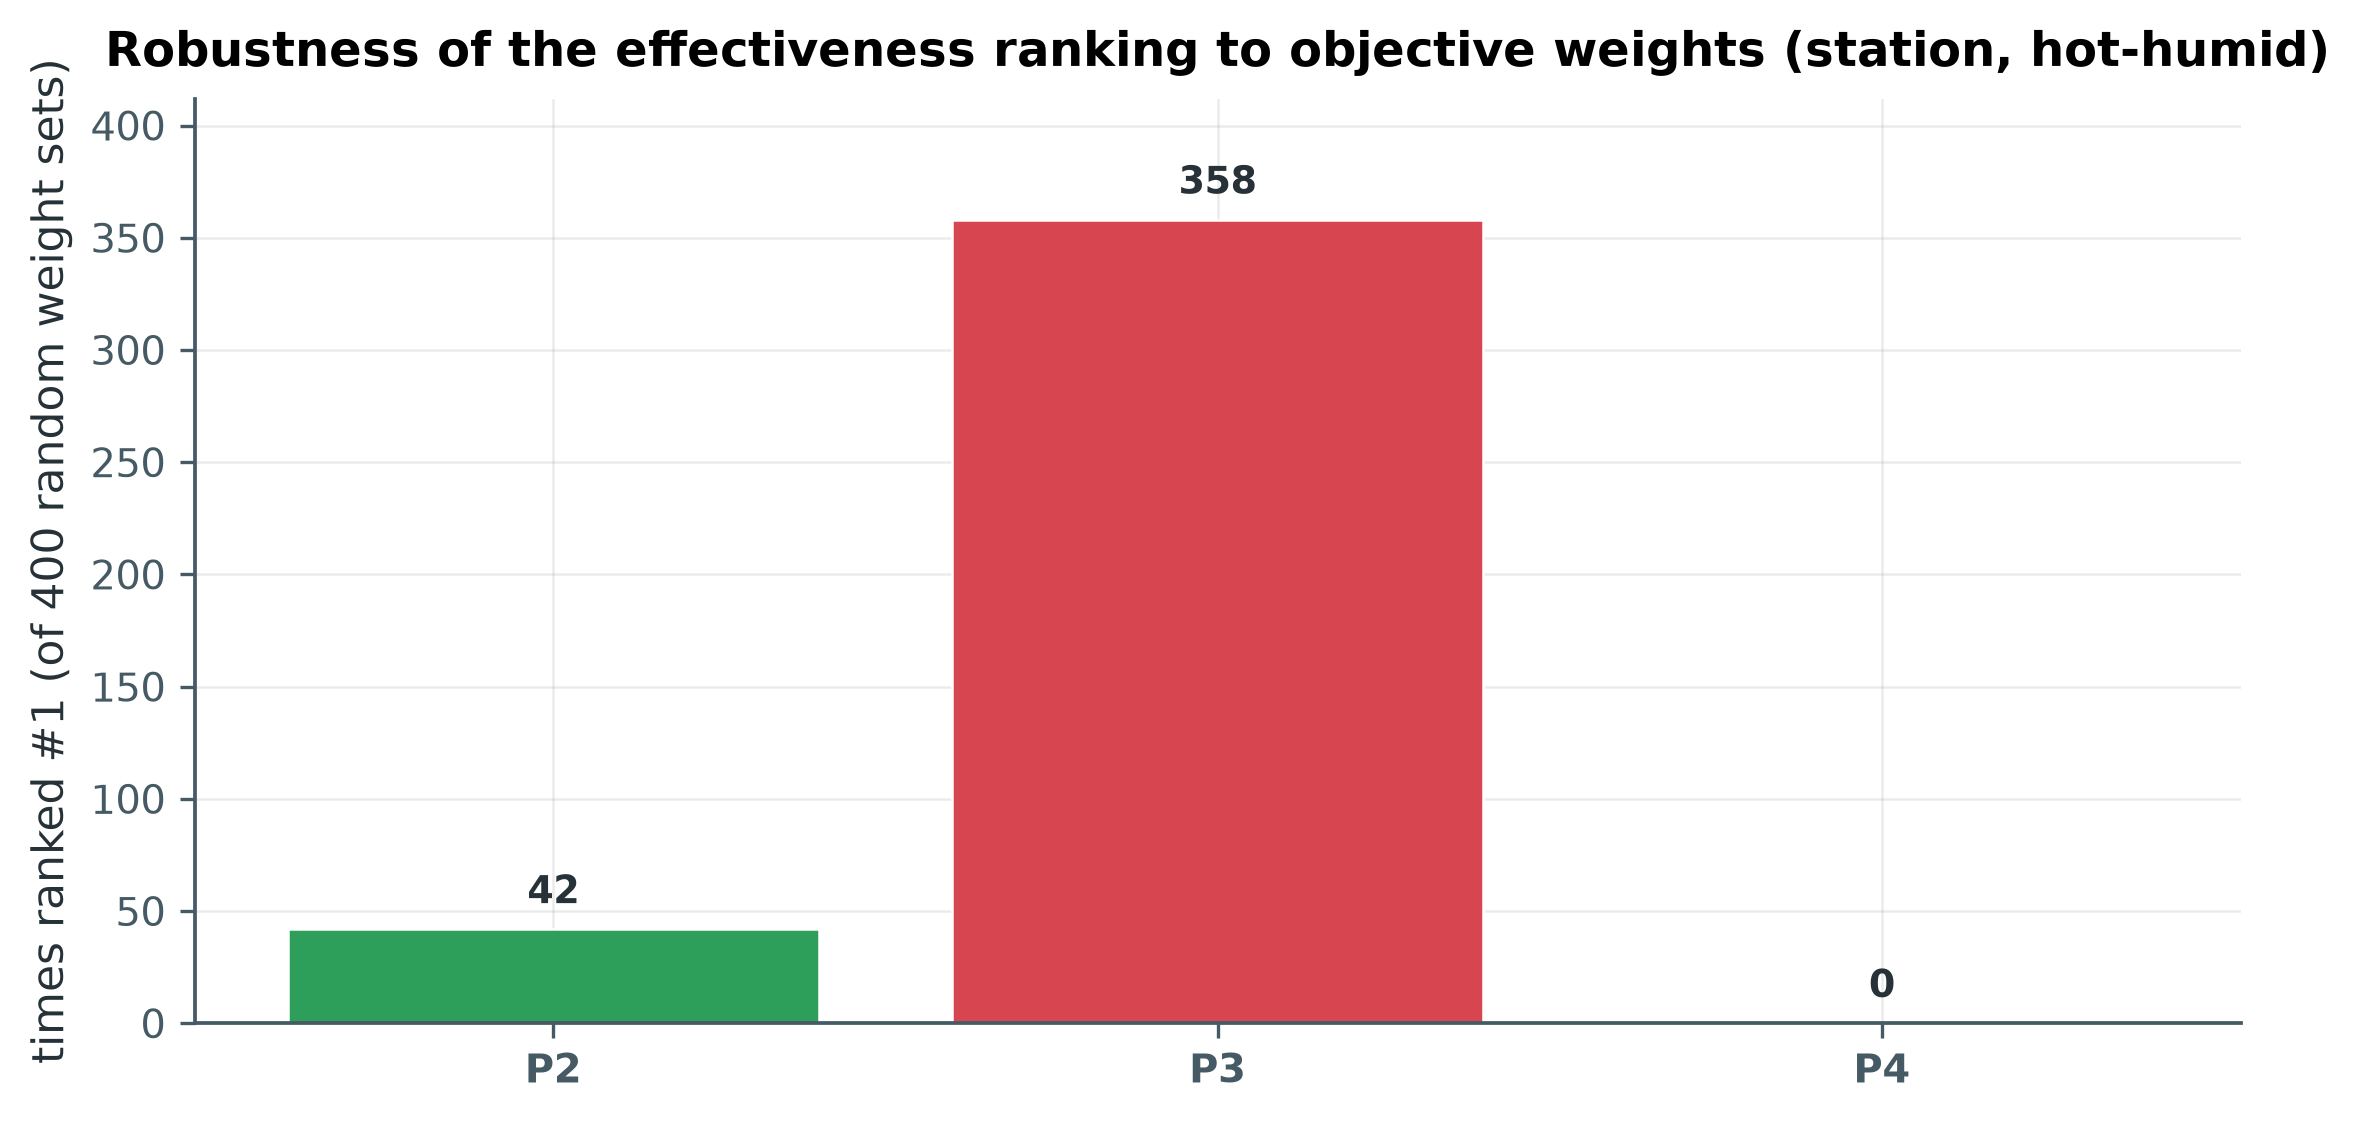
\includegraphics[width=0.62\linewidth]{fig9_weights.png}
\caption{Robustness: how often each feasible policy ranks first under 400 randomly drawn objective weights (hot-humid station).}\label{fig:weights}
\end{figure}

\textbf{Findings.} The efficiency ranking and the effectiveness ranking disagree --- and the disagreement is the message. In the dry bus stop, the fan (efficiency champion) is \emph{infeasible} at $41\degrees$C, and effectiveness selects the large cooler ($E^\ast=0.574$); in humid heat the fan is feasible again and wins ($E^\ast=0.749$). In the station, the hybrid thermostat policy wins everywhere: $E^\ast=0.729$ in hot-arid climates (first under 400/400 random weight sets) and $E^\ast=0.613$ in hot-humid (358/400, with the remainder going to always-on evaporative). Without the hard floor, doing nothing scores respectably whenever cost/energy weights are large --- which is precisely why safety must be a constraint, not a preference.

\subsection{Uncertainty quantification}
Field plant never matches the datasheet, so we re-run both climates under 400 Monte-Carlo draws that jointly perturb $UA$ ($\pm$30\%), air exchange ($\pm$40\%), thermal mass, metabolic heat, surge size, evaporative effectiveness and recirculation (ranges in Table~\ref{tab:prov}), re-simulating each policy against its own perturbed baseline. Results (Fig.~\ref{fig:mc}, Table~\ref{tab:mc}): the hybrid's saving over always-on operation has 90\% interval 37.9--47.7\% (hot-arid) and 43.3--52.8\% (hot-humid); the hybrid stays feasible in 98.8\% (hot-arid) and 100\% (hot-humid) of draws and is the lowest-energy feasible option in 98.8--100\% of them. The arid hybrid's fragility margin is real but thin: the 1.2\% of failing draws combine a weak plant (low effectiveness, poor recirculation) with the hottest afternoon. Refrigerative cooling, after calibration to Guangzhou normals, is feasible in every humid draw --- its weakness is not uncertainty but climate: it fails the floor in \emph{every} hot-arid draw. Efficiency claims that survive this test may be called robust; ours do.

\begin{figure}[H]\centering
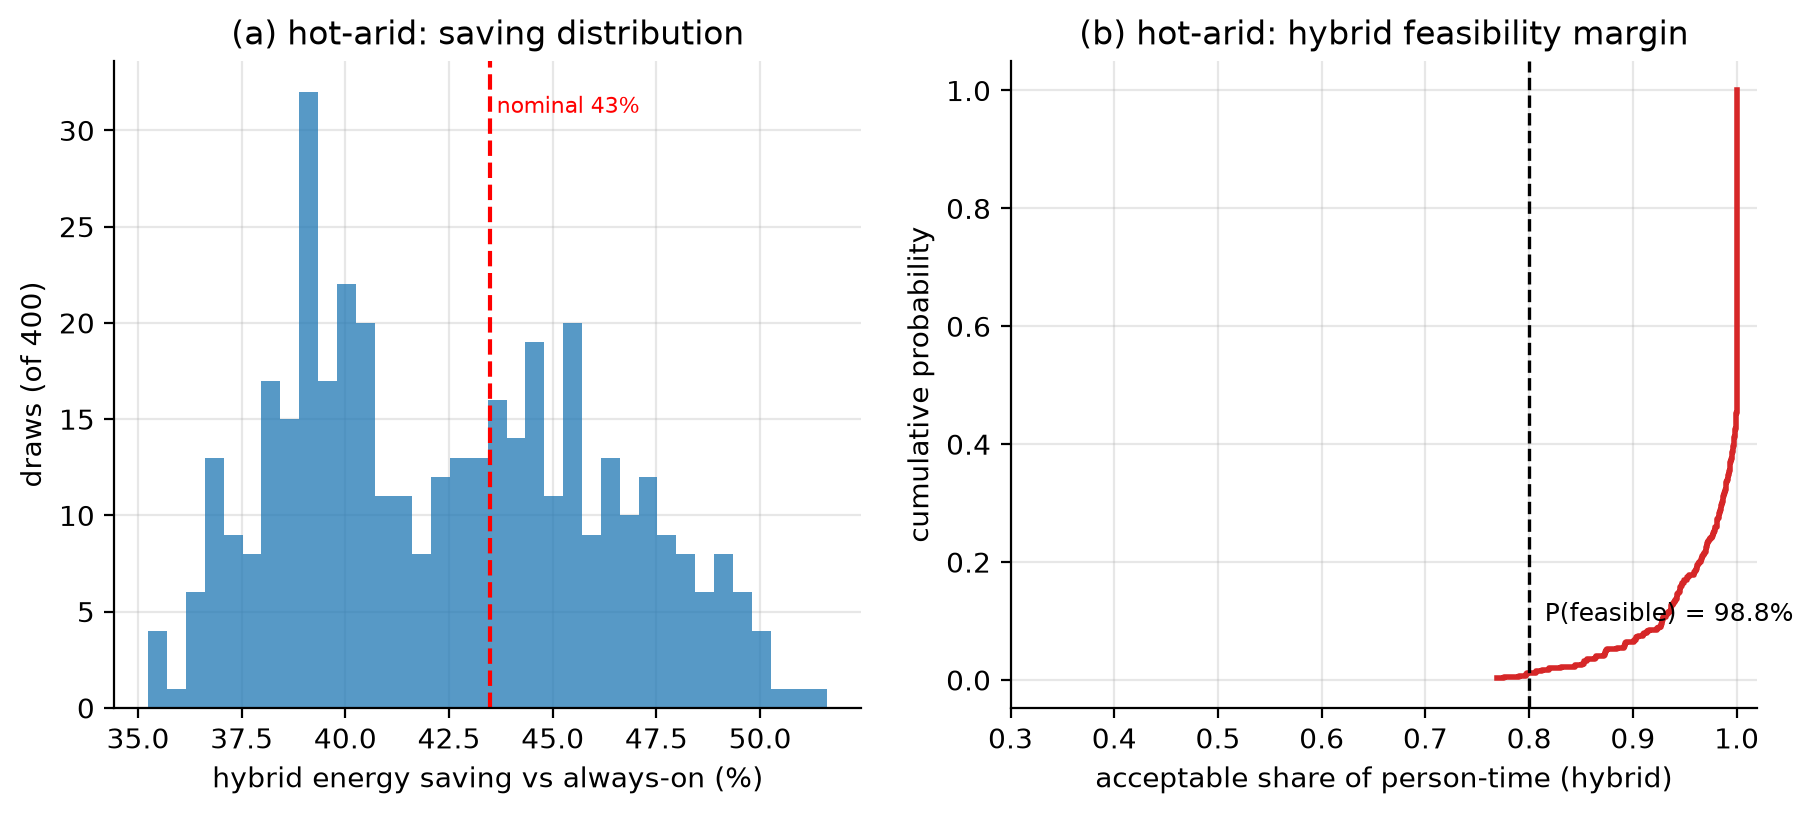
\includegraphics[width=0.98\linewidth]{fig11_mc.png}
\caption{Monte-Carlo uncertainty (400 draws). (a) hybrid energy saving vs.\ always-on (hot-arid); the dashed line is the nominal model. (b) acceptable-share distribution of the hybrid in hot-arid: 1.2\% of adverse draws dip below the 0.80 floor.}\label{fig:mc}
\end{figure}

\begin{table}[H]\centering\small
\caption{Monte-Carlo summary (400 draws; saving median with 90\% interval in parentheses).}\label{tab:mc}
\begin{tabular}{@{}lrrrrr@{}}
\toprule
Climate & saving (\%) & $P$(hybrid feas.) & $P$(refrig.\ feas.) & $P$(hybrid wins) & hybrid kWh (med.)\\
\midrule
%%TABLE_MC%%
\bottomrule
\end{tabular}
\end{table}

\subsection{Sensitivity analysis}
\begin{table}[H]\centering\small
\caption{One-at-a-time sensitivity of system B's $\DHR$; base value 50.0 (dry) and 49.5 (humid). Columns give $\DHR$ when the parameter takes its low / high value.}\label{tab:tornado}
\begin{tabular}{@{}lrrrr@{}}
\toprule
 & \multicolumn{2}{c}{Hot-arid (41\degrees C)} & \multicolumn{2}{c}{Hot-humid (33\degrees C)}\\
\cmidrule(lr){2-3}\cmidrule(lr){4-5}
Parameter & low/high & swing & low/high & swing\\
\midrule
%%TABLE_TORNADO%%
\bottomrule
\end{tabular}
\end{table}

\begin{figure}[H]\centering
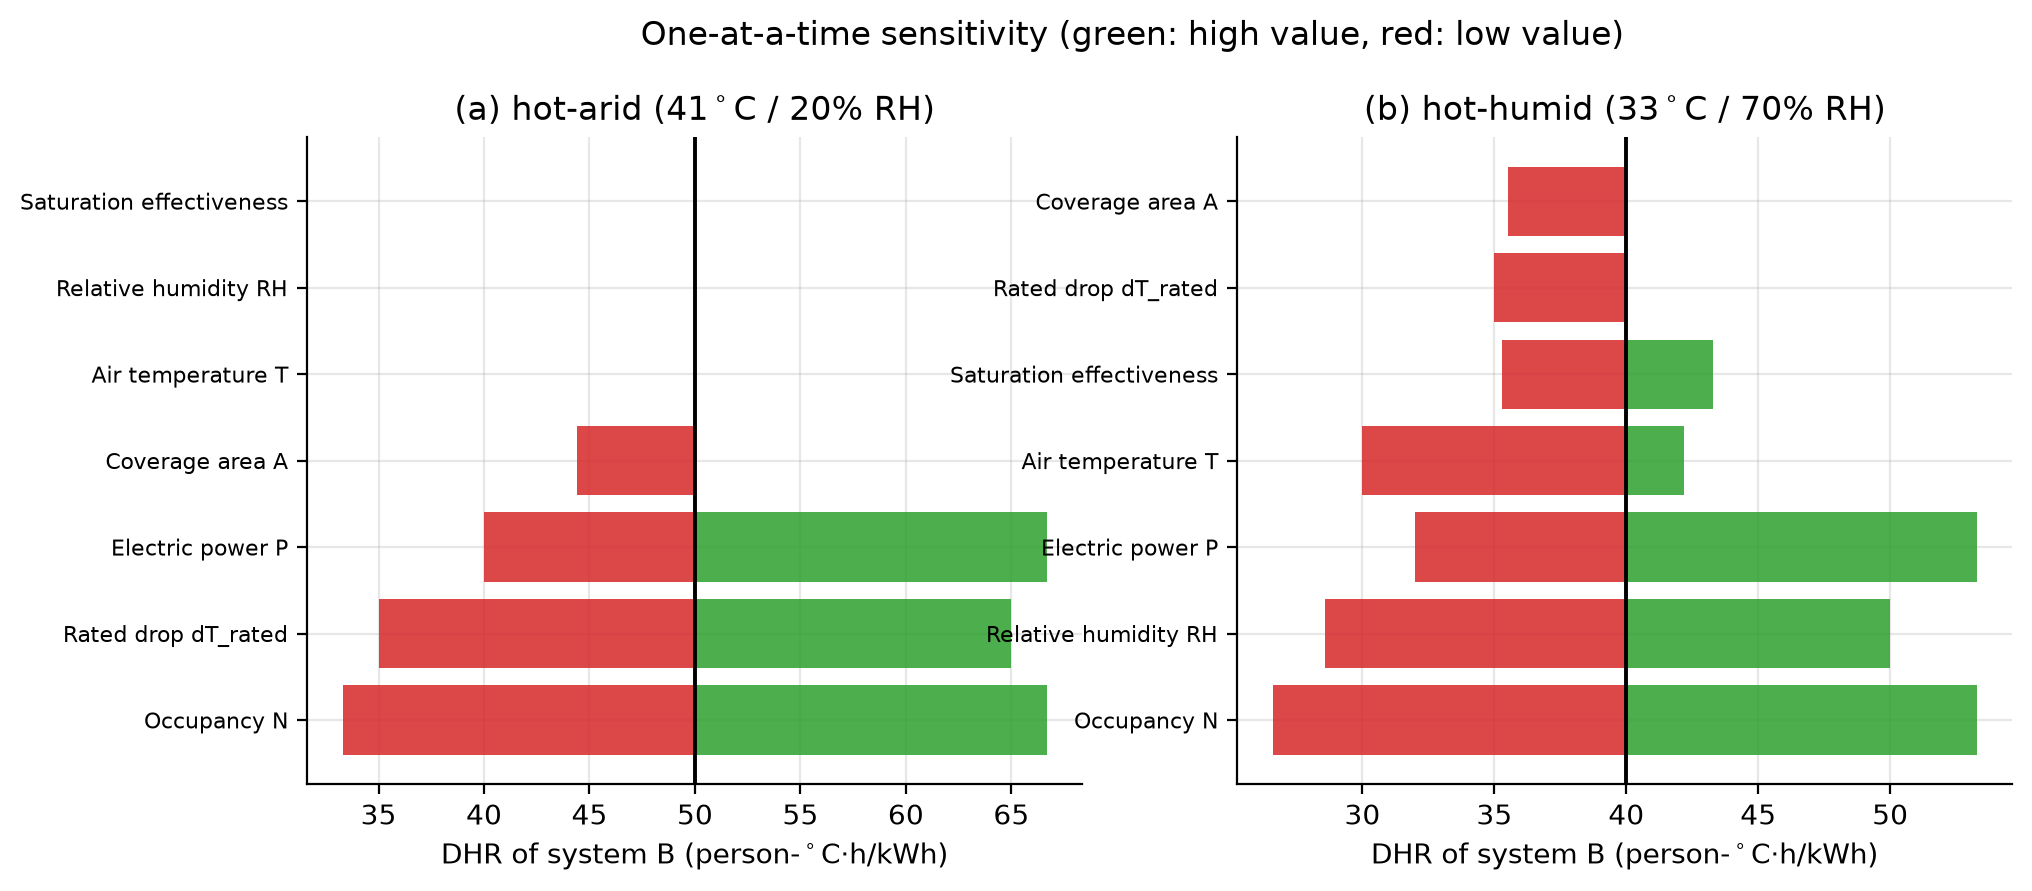
\includegraphics[width=0.97\linewidth]{fig8_tornado.png}
\caption{Tornado charts. In dry heat the evaporative system runs at its rated cap, so climate parameters swing $\DHR$ by zero; in humid heat, air temperature (through the comfort cap) and occupancy dominate, with the rated drop and humidity close behind.}\label{fig:tornado}
\end{figure}

%=====================================================================
\section{Does the Model Scale? Four Venues (Req.\ 3)}
%=====================================================================
The bus-stop equations transfer unchanged: $\DHR$ is already an \emph{intensive} metric (per kWh), and the zonal model applies wherever enclosure retains air. We evaluate four venues spanning climates, enclosure levels, and crowd densities: a Phoenix stadium concourse (hot-arid, dense), a Guangzhou rail waiting hall (hot-humid, semi-open), a Singapore outdoor patio (hot-humid, open-air), and a Honolulu airport pavilion (warm, windy). Generic systems scale with footprint: fans 4~W/m$^2$ coverage, medium evaporative 30~W/m$^2$, large evaporative 75~W/m$^2$ (fleet-scale units draw less power per m$^2$ than the shelter-class machines of Sec.~4).

\begin{table}[H]\centering\small
\caption{$\DHR$ (person-$\degrees$C$\cdot$h/kWh) and per-person relief across venues; $^\ast$ = served person below strain thresholds.}\label{tab:venue}
\begin{tabular}{@{}lrrr@{}}
\toprule
Venue & Fans & Medium evap. & Large evap.\\
\midrule
%%TABLE_VENUE%%
\bottomrule
\end{tabular}
\end{table}

\begin{figure}[H]\centering
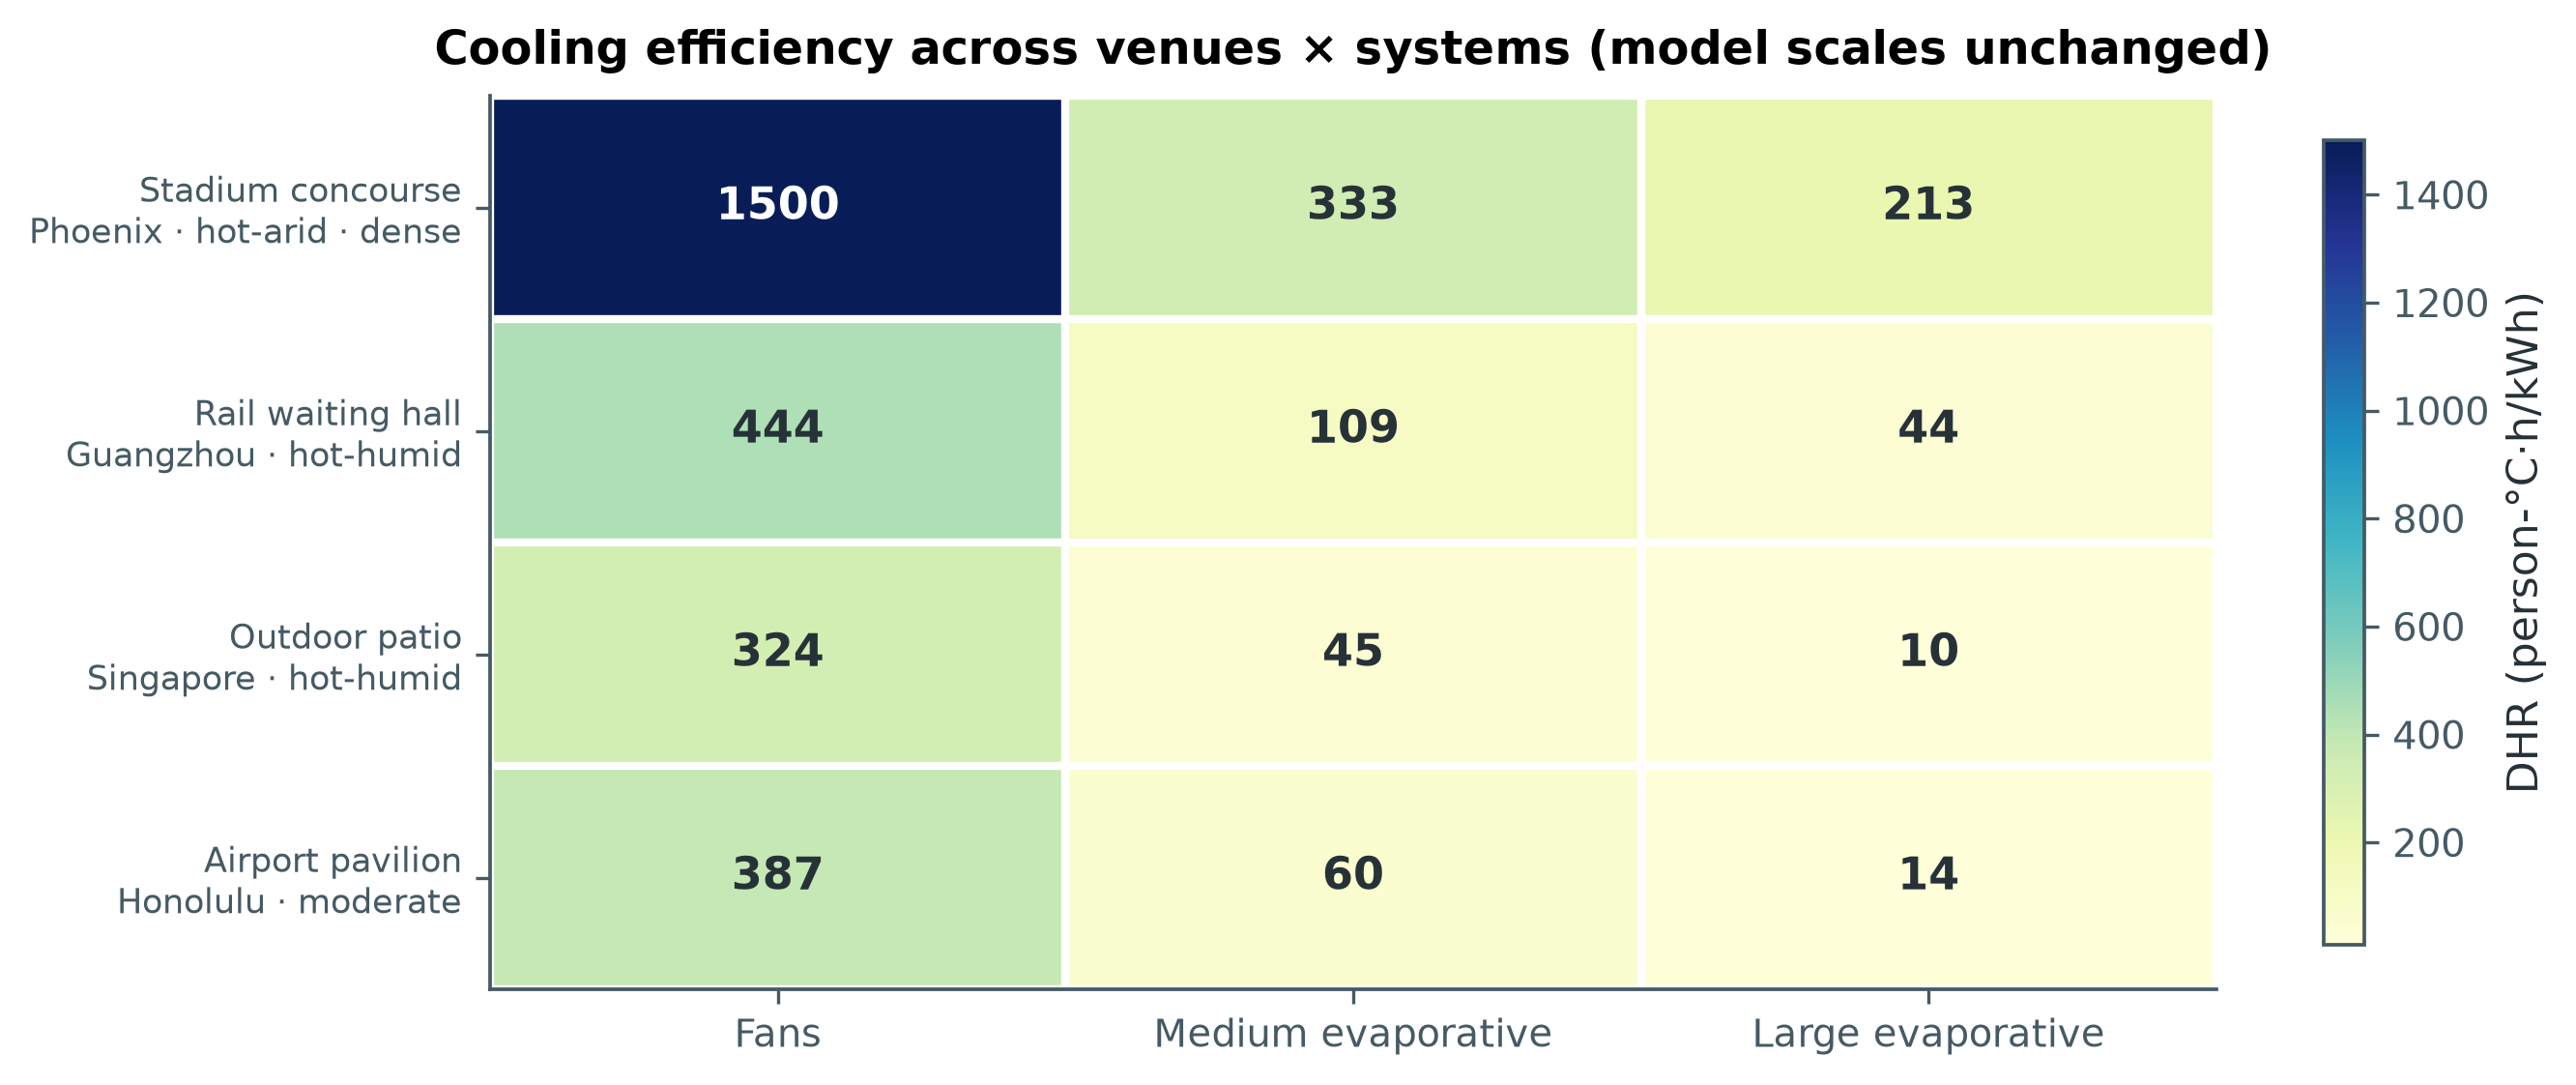
\includegraphics[width=0.9\linewidth]{fig6_venue_heatmap.png}
\caption{The same model, four venues: efficiency is set by climate (columns) and density (rows), not by venue type.}\label{fig:venues}
\end{figure}

\textbf{Robustness of scaling.} The ranking flips across climates --- fans dominate everywhere on efficiency, but the \emph{margin} changes by an order of magnitude, and only in Phoenix does the large cooler's relief ($8\degrees$C) make the difference between acceptable and unsafe waiting conditions. The model needed no re-calibration: one physics core, different boundary data.

\begin{figure}[H]\centering
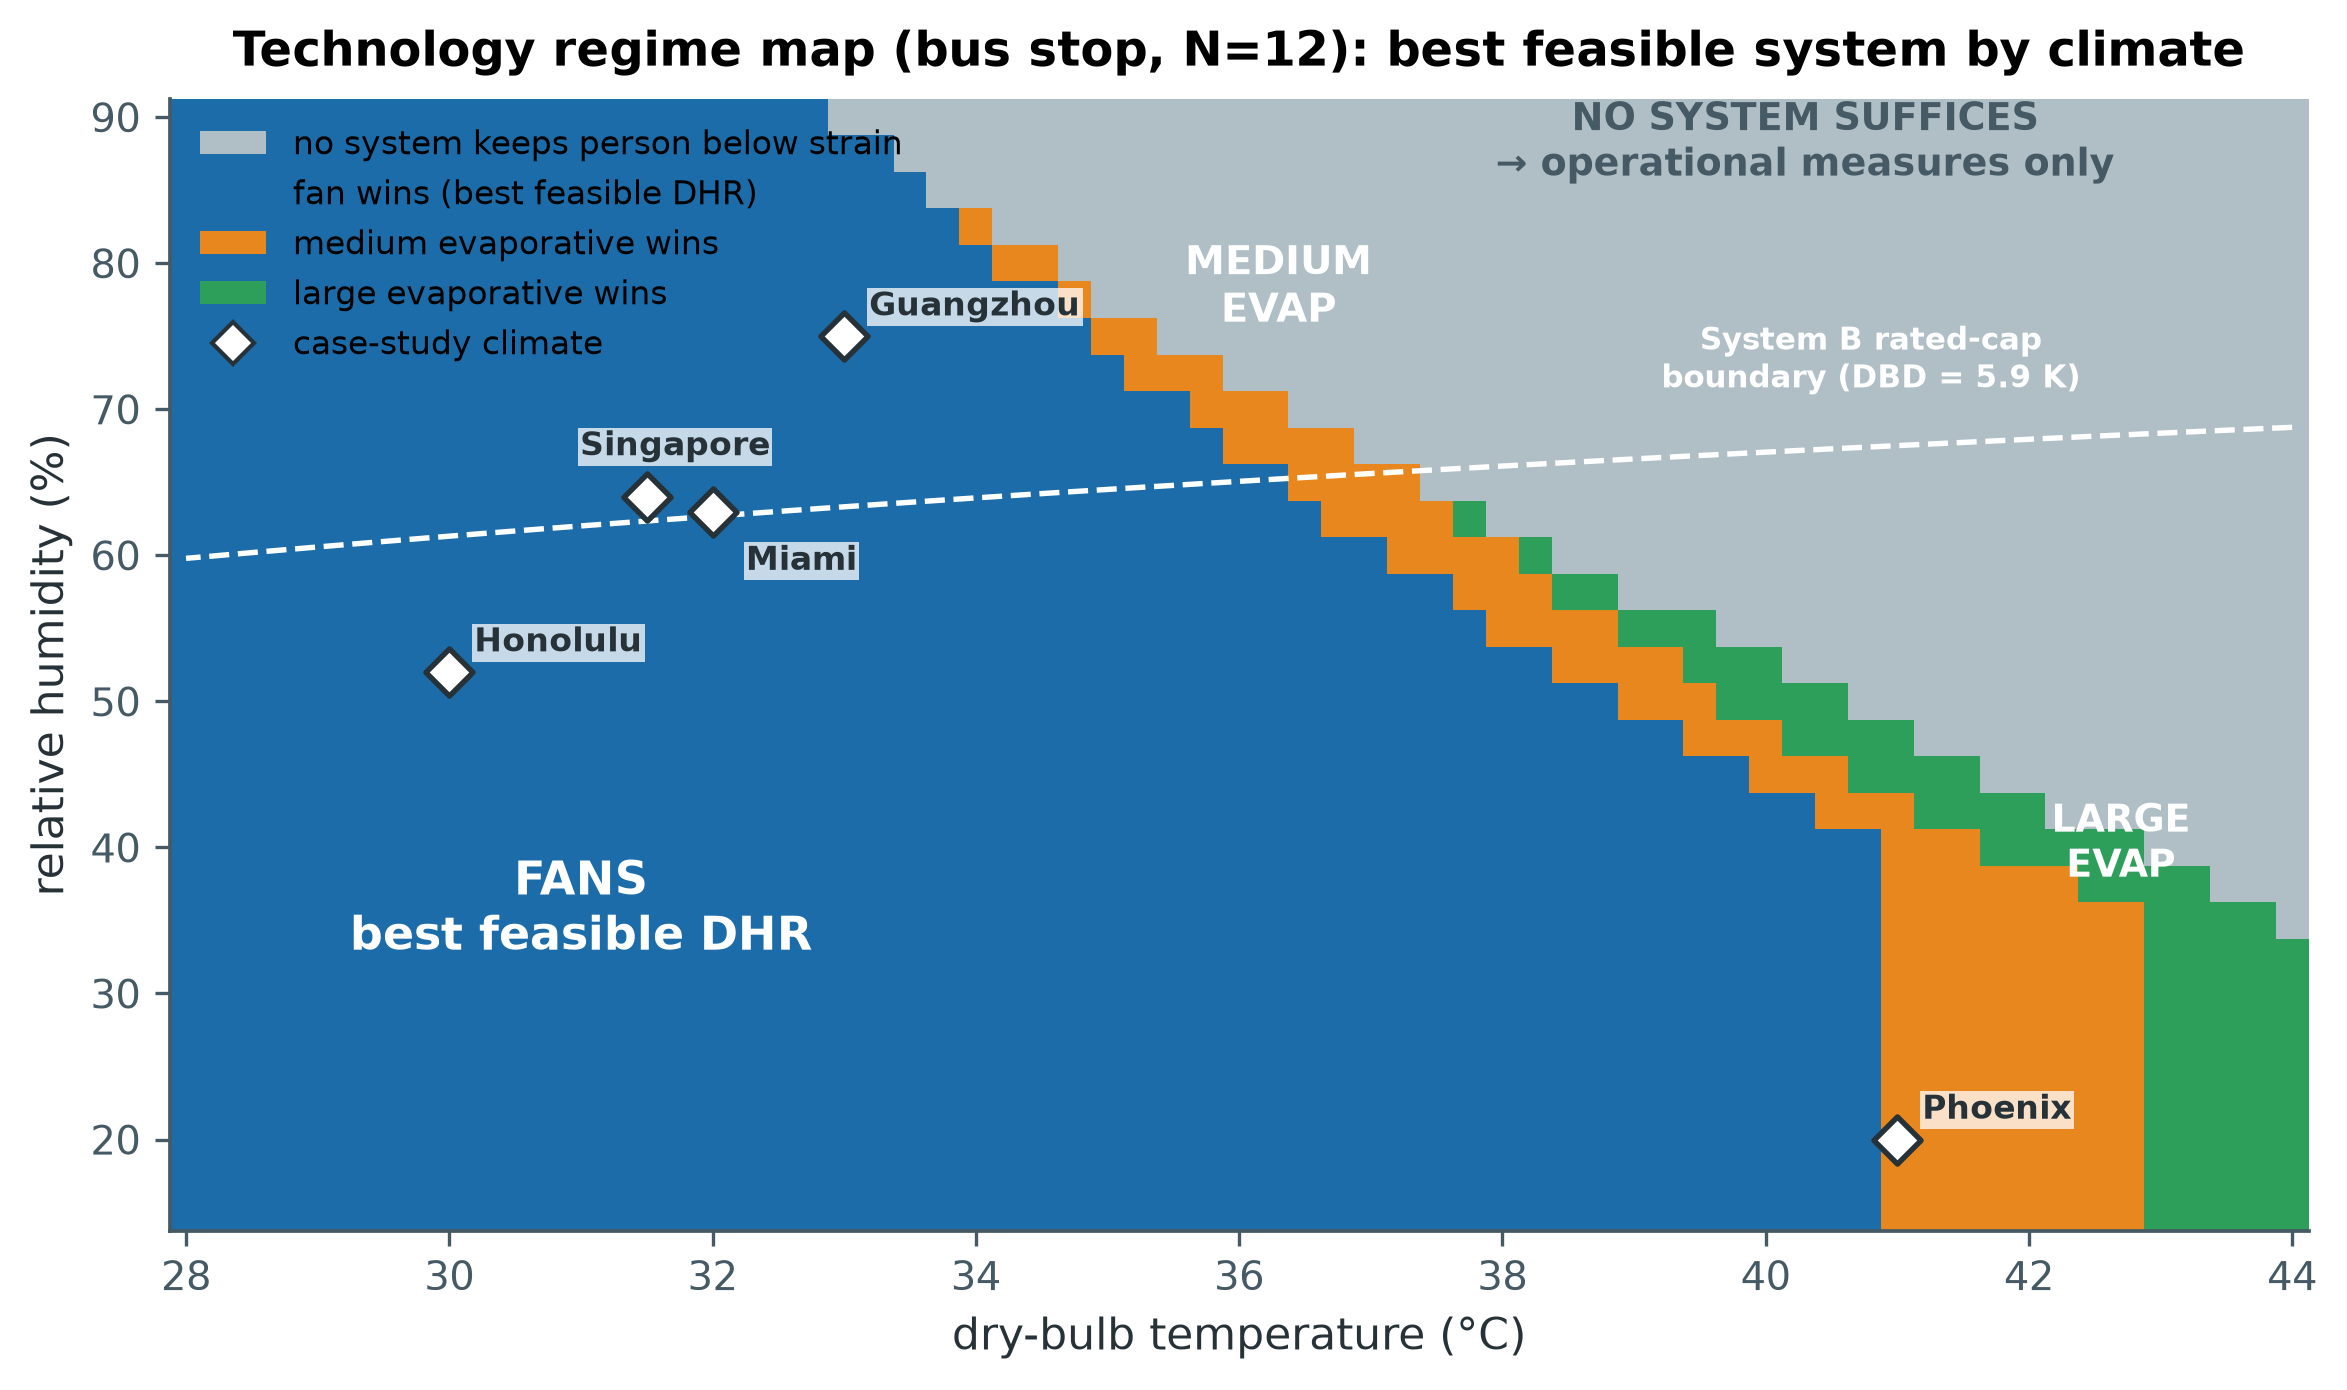
\includegraphics[width=0.86\linewidth]{fig12_regime.png}
\caption{Technology regime map: for each climate cell, the best \emph{feasible} system (highest $\DHR$ among systems keeping a served person below strain; N=12). Grey: no bus-stop-class system suffices --- only operational measures remain.}\label{fig:regime}
\end{figure}

\textbf{Where each technology wins.} The regime map (Fig.~\ref{fig:regime}) condenses the paper's practical lesson: the fan dominates routine heat everywhere; medium evaporative coolers take over in a band of very hot, very humid conditions where the fan alone cannot hold WBGT strain but the wet bulb still offers workable depression; the large cooler earns its cost only in the hot-dry corner; and a grey region of extreme humid heat admits \emph{no} bus-stop-class equipment at all --- there, only operational measures (schedule shifts, hydration stations, cooling centres) remain, which is a direct, testable planning guideline.

\textbf{Characteristics that contribute most to efficient cooling} (from Tables~\ref{tab:tornado}--\ref{tab:venue}):
\begin{enumerate}
\item \textbf{Occupancy density} --- cooling delivered per kWh scales with how many people share the footprint (top swing in both climates).
\item \textbf{Wet-bulb depression / humidity} --- zero importance in dry heat (systems run at rated cap); at Miami normals the cooler sits right at its rated-cap boundary, so air temperature, occupancy and the rated drop lead, with humidity a clear secondary driver.
\item \textbf{Rated drop vs.\ electric power} --- the efficiency lever of procurement; over-sizing wastes kWh.
\item \textbf{Coverage area} --- matters only near the crossover where the footprint stops covering everyone.
\item \textbf{Enclosure fraction and wind} --- set $\lambda$ in Eq.~(\ref{eq:ode}); the reason semi-open halls can be cooled at all.
\end{enumerate}

%=====================================================================
\section{Guidelines for Operators (Req.\ 5)}
%=====================================================================
\begin{table}[H]\centering\small
\caption{Recommended cooling strategies by climate and venue type.}\label{tab:guide}
\begin{tabular}{@{}p{2.6cm}p{5.2cm}p{6.6cm}@{}}
\toprule
Climate & Baseline (always) & Escalation tiers\\
\midrule
Hot-arid & Shade; fans over seating; misting at entries. & Tier 1: medium evaporative on thermostat. Tier 2 (WBGT${>}30$ or crowds${>}70$): large evaporative fleet + pre-cooling. Refrigerative only for recirculation-capable enclosures.\\
\addlinespace
Hot-humid & Shade; maximise air speed (fans); dehumidify where possible. & Tier 1: refrigerative units on partial recirculation. Tier 2: extend hours / add units. Evaporative as adjunct only (wet-bulb floor).\\
\addlinespace
Warm, windy & Fans and natural ventilation; shade. & Evaporative unnecessary; schedule-heavy crowd management only.\\
\bottomrule
\end{tabular}
\end{table}

\textbf{Operating strategies that balance comfort, sustainability, cost, and safety during extreme heat:}
\begin{itemize}
\item \textbf{Thermostat, not switch}: gate compressive/evaporative plant on perceived temperature with a $27.5$--$30\degrees$C hysteresis band --- $\approx$50\% energy saving at equal service (Sec.~5).
\item \textbf{Pre-cool against the timetable}: run the fleet 25--40 min before forecast surges when $T_{out}\geq32\degrees$C; thermal mass carries the hall through the pulse.
\item \textbf{Safety overrides efficiency}: when WBGT$_{\text{eff}}>32\degrees$C or $T_p>38\degrees$C, switch to always-on; during heat waves the service floor, not the kWh meter, governs.
\item \textbf{Instrument the person, not the room}: monitor WBGT and perceived temperature inside footprints; room-average temperature is meaningless in open spaces.
\item \textbf{Cheap tiers first}: fans cost $\approx$\$0.03/person-$\degrees$C$\cdot$h of relief; use expensive cooling only to close the gap the cheap tiers cannot.
\item \textbf{Carbon accounting}: at eGRID-style grid intensities (0.49--0.52 kg CO$_2$e/kWh \cite{epagrid}), the hybrid policy avoids $\approx$4.3--5.3~t CO$_2$e per 120-day season versus always-on operation --- sustainability and cost point the same way.
\end{itemize}

%=====================================================================
\section{Memorandum to the Chief Operations Officer (Req.\ 5a)}
%=====================================================================
\begin{center}
\rule{\linewidth}{0.8pt}\\[2pt]
\textbf{\large MEMORANDUM}\\[6pt]
\begin{tabular}{@{}ll@{}}
\textbf{To:} & Chief Operations Officer, HiMCM\\
\textbf{From:} & Cooling Efficiency Analysis Team\\
\textbf{Date:} & 7 November 2026\\
\textbf{Re:} & Cooling operations for the Guangzhou rail-station waiting hall (hot-humid, semi-open)\\
\end{tabular}
\rule{\linewidth}{0.4pt}
\end{center}

\textbf{Findings.} Our transient zonal model (calibrated to a $40\times12\times4$~m hall, $\approx$6 ACH air exchange, timetable surges of $\approx$70 passengers every 12--20 minutes) shows the uncooled hall peaks at $34.5\degrees$C with only 29\% of person-time acceptable --- uncomfortable, though WBGT remains below the 32$\degrees$C safety limit for solo waiting. Fans alone raise acceptability only to 46\%. Three configurations meet the 80\% service floor: (i) four large evaporative units always on --- 169.5~kWh/day, \$29.2/day; (ii) two refrigerative units always on --- 129.5~kWh/day, \$22.4/day; (iii) \textbf{fans always on plus the evaporative fleet under thermostat control with pre-cooling} --- 85.3~kWh/day, \$17.4/day, 100\% acceptable person-time. Under 400 randomly drawn objective weights, option (iii) ranks first 358 times; in hotter, drier climates the same policy wins unanimously (400/400).

\textbf{Recommendations.}
\begin{enumerate}
\item \textbf{Adopt thermostat control immediately} (ON at $T_p>30\degrees$C, OFF at $<27.5\degrees$C, plus 25--40 min pre-cool before the 07:00--09:00 and 17:00--19:00 surges): it delivers the same comfort as always-on at \textbf{half the electricity} (savings $\approx$84.2~kWh/day $\approx$ \$11.8/day $\approx$ \$1.4k per 120-day season).
\item \textbf{Keep fans running at all times}: at $\approx$\$0.03 per person-$\degrees$C$\cdot$h they are the cheapest comfort we buy, and they let the evaporative fleet cycle off sooner.
\item \textbf{Size for the wet bulb, not the datasheet}: our units deliver $6.5\degrees$C at afternoon humidity, not the rated 8$\degrees$C; procure on local wet-bulb statistics. If summer humidity keeps rising, plan a hybrid fleet (evaporative + two refrigerative units for the dehumidification margin, \$5.0/day extra).
\item \textbf{Heat-wave playbook}: when forecast WBGT exceeds 32$\degrees$C, switch the fleet to always-on, extend operating hours, and activate misting and water stations --- efficiency yields to safety above the strain line.
\end{enumerate}
\vspace{2pt}
\begin{center}\rule{\linewidth}{0.4pt}\end{center}

%=====================================================================
\section{Blog Post for the Public (Req.\ 5b)}
%=====================================================================
\begin{center}\fbox{\parbox{0.93\linewidth}{%
\textbf{\large How much cooling are we actually getting for the energy we use?}\\[4pt]
\textit{HiMCM Cooling Team $\cdot$ Public explainer}
}}\end{center}

Walk past an open freezer case in a supermarket and you can feel the answer: cold air pouring onto your ankles is money on the floor. The same thing happens, at much larger scale, whenever we cool spaces that are open to the sky --- stadium walkways, train platforms, airport gates. Some of the chill reaches you; the rest drifts off to cool... the entire neighbourhood. So how do we know whether we are getting our money's worth?

We built a simple score: for every kilowatt-hour of electricity, how many \emph{degree-hours of relief} do people actually feel? Our three biggest surprises:

\textbf{1. The humble fan is a superstar --- usually.} A small 0.25~kW fan --- about three cents an hour to run --- makes you \emph{feel} about 3$\degrees$C cooler by helping your sweat do its job. Per unit of energy, that beats big cooling machines by a factor of 2--3. But there's a catch: at 41$\degrees$C in dry heat, a fan leaves you at a dangerous 38$\degrees$C. Cheap comfort, yes --- but past a threshold, only real cooling keeps you safe.

\textbf{2. ``Up to 8$\degrees$C cooler'' depends on where you live.} Evaporative coolers work by evaporating water, and air can only swallow so much vapour. In dry Phoenix air they hit their full rating. In humid Singapore they manage about 60 percent of it --- the same machine that scores 213 in Phoenix scores just 10. The wet-bulb temperature is the ceiling; check it before you buy.

\textbf{3. \emph{When} matters as much as \emph{what}.} Cooling an empty waiting hall is pure waste. Smart controls that run the machines only when people are actually hot --- switching on near 30$\degrees$C, off near 27.5$\degrees$C, and pre-chilling before a train dumps 70 passengers onto the platform --- deliver the same comfort as running flat-out all day, on \textbf{half the electricity}.

Our advice in one line: \emph{shade and fans first; evaporative machines in dry climates; real refrigeration in humid ones; and never pay to cool an empty room.} The atmosphere is the biggest room of all --- let's stop air-conditioning it by accident.

%=====================================================================
\section{Strengths, Weaknesses, and Improvements}
%=====================================================================
\textbf{Strengths.} Physically grounded (psychrometrics, energy balance) yet person-centric; the zone ODE closes the energy balance to $10^{-3}\,\degrees$C against the analytic equilibrium; a single core scales from a bus shelter to a stadium without recalibration; efficiency and effectiveness kept separate with an explicit safety constraint; conclusions carried with grid-search optimisation, robust selection and Monte-Carlo uncertainty; all results reproducible from code.

\textbf{Weaknesses.} Comfort thresholds (27/30/38$\degrees$C) and footprints are population-level estimates; WBGT is approximated from dry-bulb/wet-bulb rather than measured globe temperature; radiation loads are coarsely lumped; economic parameters are illustrative; CFD-level airflow inside footprints is ignored.

\textbf{Improvements.} Calibrate $\kappa$, $\lambda$, footprints with field data (one instrumented shelter suffices); replace the comfort cap with PMV \cite{fanger}; optimise the thermostat band and pre-cool duration against the full timetable; multi-year weather ensembles for robust procurement.

%=====================================================================
\begin{thebibliography}{9}
%=====================================================================
\bibitem{ashrae} ASHRAE. \emph{ASHRAE Handbook---Fundamentals}. Atlanta: ASHRAE, 2021.
\bibitem{ashrae55} ANSI/ASHRAE. \emph{Standard 55-2020: Thermal Environmental Conditions for Human Occupancy}. Atlanta: ASHRAE, 2020.
\bibitem{acgih} ACGIH. \emph{TLVs and BEIs: Heat Stress and Strain}. Cincinnati: American Conference of Governmental Industrial Hygienists, 2017.
\bibitem{sherwood} Sherwood, S.~C., and M.~Huber. ``An adaptability limit to climate change due to heat stress.'' \emph{PNAS} 107.21 (2010): 9552--9555.
\bibitem{fanger} Fanger, P.~O. \emph{Thermal Comfort: Analysis and Applications in Environmental Engineering}. Copenhagen: Danish Technical Press, 1970.
\bibitem{stull} Stull, R. ``Wet-bulb temperature from relative humidity and air temperature.'' \emph{J. Appl. Meteor. Climatol.} 50.11 (2011): 2267--2269.
\bibitem{epa} U.S. EPA. \emph{Excessive Heat Events Guidebook}. EPA 430-B-06-005, 2006.
\bibitem{comap} COMAP. ``2026 HiMCM Problem B: Air Conditioning the Environment.'' COMAP, Inc., 2026.
\bibitem{doe} U.S. Department of Energy, EERE. \emph{Room Air Conditioner Standards: Technical Support Document}. Washington, DC: DOE, 2016.
\bibitem{eia} U.S. Energy Information Administration. \emph{Electric Power Monthly}. Washington, DC: EIA, 2025.
\bibitem{epagrid} U.S. Environmental Protection Agency. \emph{Emissions \& Generation Resource Integrated Database (eGRID)}, 2022 data. Washington, DC: EPA, 2024.
\bibitem{noaa} NOAA National Centers for Environmental Information. \emph{U.S. Climate Normals 1991--2020}. Asheville, NC: NCEI, 2021.
\bibitem{greenchill} U.S. EPA GreenChill Partnership. \emph{Supermarket Refrigeration Audits and Case Studies}. Washington, DC: EPA, 2013.
\end{thebibliography}

\newpage
%=====================================================================
\section*{Appendix A: Full bus-stop results}
\addcontentsline{toc}{section}{Appendix A: Full bus-stop results}
%=====================================================================
Table~\ref{tab:busfull} reports all 36 combinations of climate, occupancy and system for the bus stop (Fig.~\ref{fig:bus} plots the summary).
\begin{table}[H]\centering\small
\caption{Complete bus-stop results ($\DHR$ in person-$\degrees$C$\cdot$h/kWh; $r$ = felt relief; $T_p$ = perceived temperature of a served person).}\label{tab:busfull}
\begin{tabular}{@{}llrrrrr@{}}
\toprule
Climate & System & $N$ & $r$ (\degrees C) & served & $T_p$ (\degrees C) & $\DHR$\\
\midrule
%%TABLE_BUSFULL%%
\bottomrule
\end{tabular}
\end{table}

\newpage
%=====================================================================
\section*{Report on the Use of AI Tools}
\addcontentsline{toc}{section}{Report on the Use of AI Tools}
%=====================================================================
\textit{(Per contest rules this report does not count toward the 25-page limit.)}\\[4pt]
During preparation of this solution we used an AI assistant (ZCode environment, GLM model) for: (i) suggesting the structure of the efficiency/effectiveness framework and the psychrometric formulations; (ii) generating the Python simulation code and LaTeX tables/figures from our model specifications; (iii) assisting with the drafting and language of this manuscript. All assumptions, parameter choices, and modelling decisions were reviewed, verified, and where necessary corrected by the team (e.g., the wet-bulb solver's bisection sign and integral units were audited against hand calculations). The team takes full responsibility for the final content and acknowledges the assistance in accordance with the contest's AI-use disclosure policy.

\end{document}
